%###########################################################################################
% TYPE DE DOCUMENT
%###########################################################################################
% pour les soucis avec les MAC
%!TEX encoding = UTF-8 Unicode
%
\documentclass[a4paper, 12pt, titlepage, twoside]{these}

\usepackage[english]{minitoc}
\usepackage{minted}

%\usepackage[avantgarde]{quotchap}

\graphicspath{%
{/home/manuel/DIVERS/Graphes/Memoire/}%
{/home/manuel/DIVERS/Graphes/StageM2/}%
}%

\newcommand{\titree}{}%
\newcommand{\auteur}{Manuel Duarte}%

%pour les choix des styles des codes colorisés avec minted
\usemintedstyle{perldoc}%

\setcounter{minitocdepth}{1}

\begin{document}
\dominitoc
\newcommand{\testtitle}{true}
\renewcommand{\testtitle}{false}
\renewcommand{\labelitemi}{\textbullet} % changer les items des listes
\begin{sloppypar}
\tableofcontents\thispagestyle{these}
%\twocolumn
\renewcommand{\labelitemi}{\textbullet} % changer les items des listes
\ps{Galaxy groups in the SDSS}
\bartchapterimage{rampressure}
\bartthumb{thumb_rampressure}
\cs{Luminosity function}
\fs{Determine the LF}

\postit{There is very lot of words in this note but I can't stop
to write, else the world will end !}{5}

When we want to compare the results from our galaxy group finder to other existing algorithms, we have to compare a flux limited
catalogue with our algorithm. But as said before, our algorithm works on a double complete sample of galaxies. So, we need to develop
a flux limited version of our algorithm.

The problem when working with a flux limited sample of galaxies is that we must correct for missing galaxies. The galaxies observed
by the survey can be seen just when they are brighter than a luminosity limit which depends on the redshift (the distance of the
galaxy). We can determine this luminosity easily by the theory:
\begin{eq}
    L_{\mathrm{lim}}\pg{z}\pd={{\pg\frac{d_{\rm{lum}}\pg{z}\pd}{10pc}\pd}^2}\num{10}^{\num{0.4}\pg{M_{\odot}-m_{\rm{lim}}}\pd}
\end{eq}
with $m_{\mathrm{\lim}}$ the magnitude limit of the survey and $M_{\odot}$ the absolute magnitude of the sun, all in the same band
filter. This luminosity is in unit of sun luminosity. In ours groups, when they are at a distance above the distance limit to see
galaxies with the luminosity threshold of the catalogue, some galaxies are missing because they can't be seen. In order to correct for
the number of missing galaxies, we have to know the distribution of galaxy luminosities. With this luminosity function (LF), we can
calculate the ``fraction'' of galaxy luminosities in mean that we can see:
\begin{eq}\label{eq:correc}
    f\pg{L_{lim}{\pg{z}\pd}}\pd=\frac{\int_{L_{lim}\pg{z}\pd}^{\infty}L\phi{\pg{L}\pd}\dd{L}}{\int_{L_{thres}}^{\infty}L\phi{\pg{L}\pd}\dd{L}}
\end{eq}
where $\phi\pg{L}\pd$ is the LF\@. So determining this LF is useful to correct for missing galaxies.

But, as we expect with the goal of this thesis, it's clear for us that properties of galaxies depend on the environment. So the
luminosity function may probably depend on the host halo. The LF have to depend on different characteristics of the halo. The unique
``observable'' property is the virial mass so we want that the LF depends on it. This is the better way to correct for the
incompleteness of groups, with a particular correction for each group. \com{Put something in order to justify physically this
dependence on the halo mass!} Resulting from this idea, the LF used in (\ref{eq:correc}) becomes a conditional LF, which is the LF in
groups of a given halo mass:
\begin{eq}
    \phi\pg{L}\pd\rightarrow\phi\pg{L|M}\pd%
\end{eq}
\postit{There is very lot of words in this note but I can't stop
to write, else the world will end !}{5}

In galaxy groups, we separate galaxies in two classes: centrals and satellites. Centrals are expected to be the most massives
galaxies in groups, and consequently, it's probable that the central is the brighter galaxy. A consequence is that if we can't see
the central galaxy, we can't see other galaxies in the group and the correction is not needed because we don't know how to correct
for incompleteness. So for the correction we just need to constrain the distribution of luminosities in satellite galaxies.

In practice, we have to choose a functional for this conditional luminosity function (CLF) which can be easily fitted and integrated
to determine the correction factor in our group luminosities. In studies of the galaxy sample from the SDSS survey as in
\citet{Blanton+05}, the LF has been well fitted by a double Schechter functional form which can be written:
\begin{eq}\label{eq:dblsch}
    \phi\pg{L}\pd=\pg{\phi_1^*{\pg{\cfrac{L}{L_*}}\pd}^{\alpha_1}+\phi_2^*{\pg{\cfrac{L}{L_*}}\pd}^{\alpha_2}}\pd\exp\pg{-\pg{\cfrac{L}{L_*}}\pd}\pd%
\end{eq}

Now we assume that the CLF have the same form that (\ref{eq:dblsch}). The dependence on the halo mass $M$ is taken with the
parameters of the double Schechter (DS). For example $\alpha_1\rightarrow\alpha_1\pg{M|\theta}\pd$, where the functional form of
this dependence is not given explicitly here, and $\theta$ is a set of parameters relative to the function used to describe the
dependence with halo mass. The number of parameters in $\theta$ can vary greatly, depending on the function used.

The form of this dependence can't be determine in advance when we want to fit the CLF on the data. For example in the SDSS, we have
to know in advance the properties of the groups in order to choose a certain dependence for the parameters of the DS with the virial
mass. So, for testing the viability of this method, we have to select a functional that describes correctly the modulation of the
parameters with the halo, and samples of galaxies that can give us this information are present in outputs of semi-analytical models
(SAM). In such samples, we know in which group a galaxy is, and the virial mass of the host halo is known too. To validate this
method of correction for incompleteness, we can test it in mock galaxy catalogues.

\fss{Estimating parameters}
We need to use a method for estimating the parameters that fit well the data (real or simulated). When working with distribution
function, it is common and better to use the maximum likelihood estimation defined as:
\begin{eq}\label{eq:like}
    \mathcal{L}\pg{\theta|X}\pd=\prod_i{p_i\pg{X_i|\theta}\pd}
\end{eq}
where $X$ is the set of data (in our case the luminosity $L$) and $\theta$ the set of parameters of the model that have to be
estimated.

If we consider Bayesian statistics, the likelihood is defined as $p\pg{X|\theta}\pd$ and it seems to be incoherent. But using the
Bayes's theorem, we can see that \emph{our} likelihood is in reality the posterior distribution which is proportional to the
likelihood in the definition of Bayesian statistics, multiply by a prior. But we don't have any prior on the parameters distribution
(which can be discussed\ldots). So, if we take a constant for the prior (probability equal for each parameter), we get same results.

It's more convenient to use the logarithm of the likelihood in order to prevent numerical problems when calculating the likelihood.
The product in (\ref{eq:like}) becomes at this moment a sum, and the computation is simplified. It's easier too to minimize a
function numerically so we rewrite it.
\begin{eq}\label{eq:loglike}
    -\log\mathcal{L}\pg{\theta|X}\pd=-\sum_i{\log\pg{p_i\pg{X_i|\theta}\pd}\pd}
\end{eq}

We define $p_i\pg{X_i|\theta}\pd$ as the probability to get the value $X_i$ given the parameters $\theta$, so it's the probability
density. To determine this density, we need to calculate the number of ``points'' in the sample which are between $X_i$ and
$X_i+\dd{X_i}$ compare to the total number of points in the set $X$:
\begin{eq}
    p_i\pg{X_i|\theta}\pd\dd{X_i} = \cfrac{\dd{N_i}}{N_{\mathrm{tot}}}
\end{eq}

By definition of the CLF, which is the number of galaxies by unit of volume comprised between $L$ and $L+\dd{L}$ at a given halo
mass $M$, we can write:
\begin{eq}
    \dd^2{N}=\phi\pg{L|M}\pd\dd{L}\dd{V}
\end{eq}
Summing on all the volume in which we are working, we get:
\begin{eq}
    \dd{N}=\phi\pg{L|M}\pd\dd{L}
\end{eq}
\com{Because we are working in limited volume region, we can rewrite the probability density as:
\begin{eq}
    p_i\pg{L_i|\theta}\pd\dd{L_i}\dd{V} = \cfrac{\dd^2{N_i}}{N_{\mathrm{tot}}}
\end{eq}}
So we can write:
\begin{eq}
    p_i\pg{L_i|\theta}\pd\dd{L_i} = \cfrac{\phi\pg{L_i|M}\pd\dd{L_i}}{N_{\mathrm{tot}}}
\end{eq}
and the total number of galaxies is just:
\begin{eq}
    N_{\mathrm{tot}}=\int_{L_{\mathrm{thres}}}^\infty{\phi\pg{L|M}\pd\dd{L}}
\end{eq}
In this way, the density probability for the DS can be written:
\begin{eq}
    p_i\pg{L_i\left|\alpha_1, \alpha_2, M_*, \cfrac{\phi_2^*}{\phi_1^*}\right.}\pd=\cfrac{\pg{{\pg{\cfrac{L}{L_*}}\pd}^{\alpha_1}
    +\cfrac{\phi_2^*}{\phi_1^*} {\pg{\cfrac{L}{L_*}}\pd}^{\alpha_2}}\pd\exp\pg{-\pg{\cfrac{L}{L_*}}\pd}\pd}{\pg{\Gamma\pg{1+\alpha_1,
    \cfrac{L_{\mathrm{thres}}}{L_*}}\pd+\cfrac{\phi_2^*}{\phi_1^*}\Gamma\pg{1+\alpha_2,\cfrac{L_{\mathrm{thres}}}{L_*}}\pd}\pd}
\end{eq}
where $\Gamma\pg{a,x}\pd=\int_x^{\infty}e^{-t}{t^{a-1}}\dd{t}$ is the incomplete gamma function.

The principle of the estimation by the method of the maximum likelihood is that when we maximize the likelihood relatively to the
parameters $\theta$, we get the maximum of probability, likelihood, of having the parameters that correspond denoted $\hat{\theta}$.
The parameters $\hat{\theta}$ are the parameters that best fit the data according to the functional form assumed for the CLF.\@
Numerically we minimize the equation (\ref{eq:loglike}).

There are many ways of doing such a minimization. When the probability density isn't too complex, $\hat{\theta}$ can be determined
analytically. But in this case, with the DS, the incomplete gamma function prevent us to do it in this way. So we are constrained to
use numerical methods in order to minimize the likelihood. Many algorithms exist to do this job like Powell's method,
Newton-Raphson's method, etc\ldots, but they share the same problem: when they find a minimum, we can't know if it is the global
minimum or if it is a local minimum. The result depends on the initial starting point of the algorithm in the parameter space. Some
other methods try, using Monte-Carlo methods, to do a better exploration of this parameter space, allowing some ``jumps'' to other
regions in order to see if there isn't a best minimum near. An example of such an algorithm is the simulated annealing method which
implement the cooling of a material where the function to minimize becomes the energy of the system and a fictive temperature $T$ is
introduce to allow some temperature jumps. But it is not always sure that we get the global minimum. Moreover, we can't easily
determine errors on the estimation of the parameters, except using bootstraps or jackknife techniques which need many estimation
of the parameters varying the sample which may be expensive in calculation time.

We have chosen to use the Markov Chains Monte Carlo method (MCMC) to minimize our function. This method is the better in all the
universe. \com{Explain why!}. We can estimate easily with results of the algorithm the errors on the parameters.

We will now resume the result of works on mock catalogues of our method of estimating the CLF.\@

\fss{Tests on mock catalogues}
There is two steps in order to determine the dependence on the halo mass of the parameters of the DS model. First, we have to
determine what is the best functional form to fit this dependence which can be done on a complete sample of galaxy. Secondly, see if
we can recover this parametrisation and modulation with a flux limited sample of this galaxies to know if the method works well when
applied in a real survey.

\fsss{Complete sample}
In order to determine the dependence on the halo mass of the parameters, we use a complete sample of galaxies taken from the outputs
of the SAM of \citet{Guo+11} applied on dark matter halos from the Millennium II run. We limit our sample of galaxies from this
catalogue to galaxies with a luminosity such that the absolute magnitude in the $r$ band is $M_r<-12$. For each galaxy, we have the
virial mass of the halo which contains this galaxy. Our complete sample is defined just as this galaxy catalogues from
\citet{Guo+11} with the truncation on the data through the $r$ band magnitude.

First, we determine what is the best model for the ``total'' CLF, \textit{i.e.} the LF when we don't do a segregation with the halo
mass. We have tried to adjust a simple Schechter and a double Schechter. Results are shown on figure (\ref{fig:fitguo}).
\begin{figure}[ht]
    \centering
    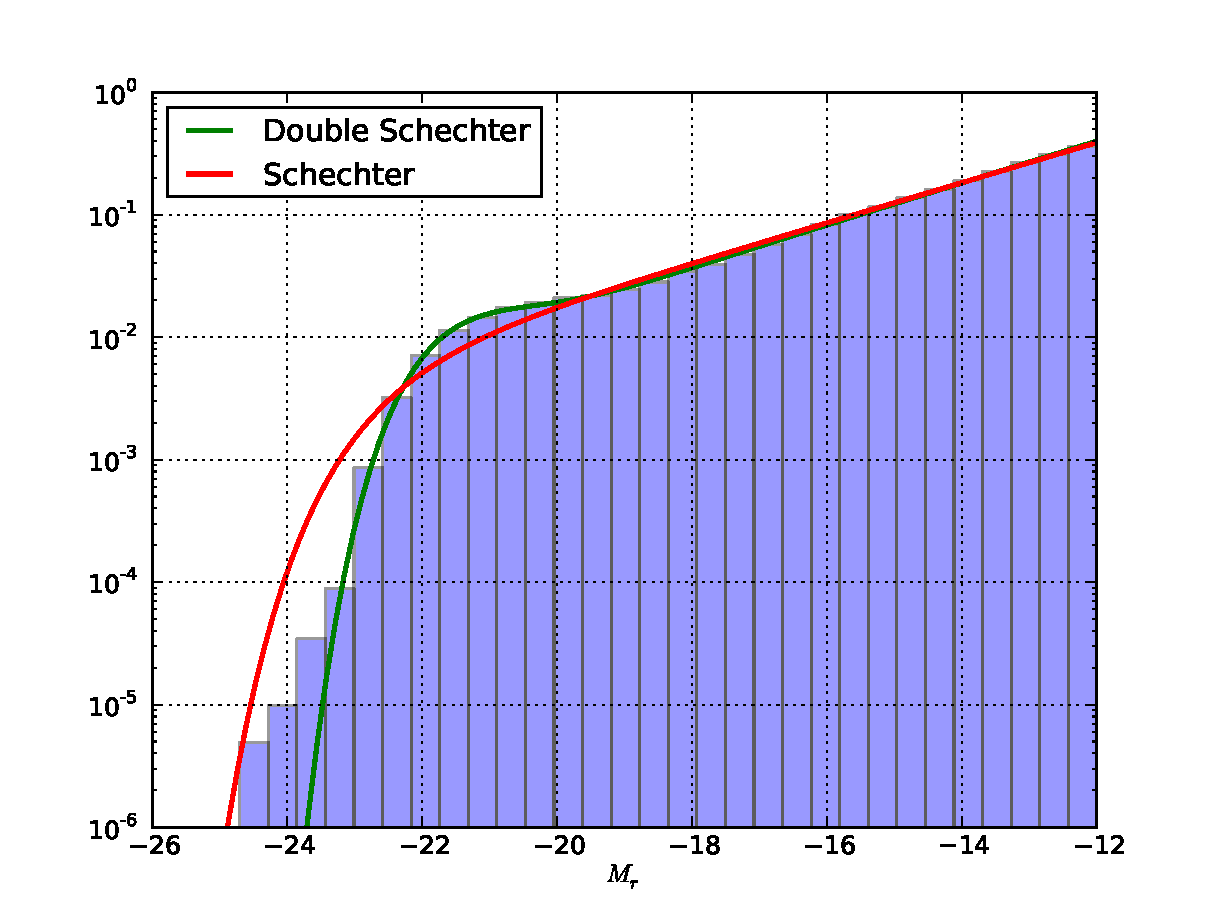
\includegraphics[width=0.5\linewidth]{MCMCfitGUO}
    \caption{\footnotesize{}Results of the fit on the data in blue with a Schechter distribution in red and a double Schechter
    distribution in green. The double Schechter fit is better because this form allow to constrain the two galaxy populations we
    can see in our sample: a low population with high slope and a brighter population with a more little slope in absolute
    value.}
\label{fig:fitguo}
\end{figure}
We can see that the minimization works well because the fit seems to be good enough in the figure. The double Schechter fits better
the data than the simple Schechter because we can constrain with this form the two populations of galaxies in the sample from the
\citet{Guo+11} SAM.\@ We see that there is a low population with high slope and a brighter population with a slope more little.
Differences with the data at luminous galaxies is due to the fact that the number of galaxies with $M_r<-24$ is very low, in some
bins there is just one galaxy. But we need a quantitative proof of this fit. We use for that the Kolmogorov-Smirnov test ans the
P-Value associated.\com{TODO:\@ KS test on the fit in order to get a good idea of the robustness of the fit.}
\begin{figure}[H]
    \centering
    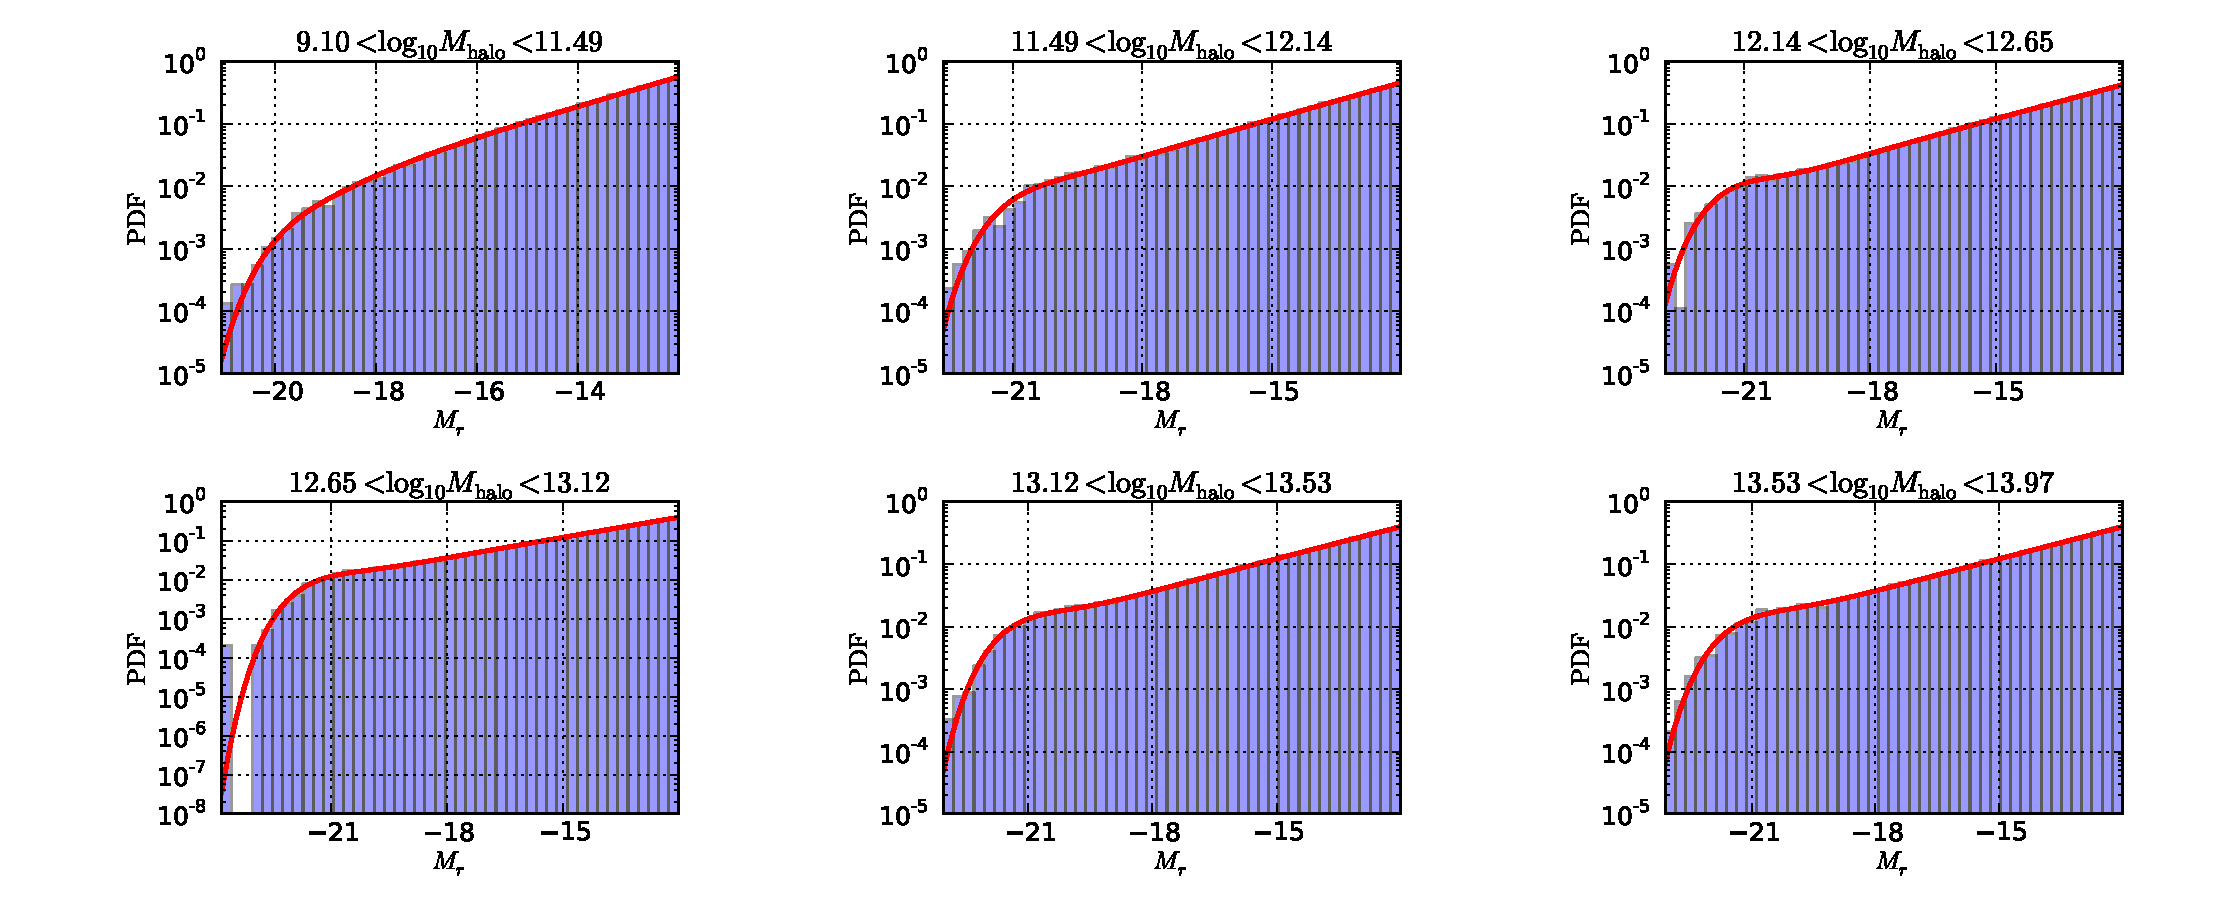
\includegraphics[width=\linewidth]{FitDblSchechterGuo}
    \caption{Results of the fit for the double Schechter distribution in different bins of halo mass. In blue the
    PDF of the data, and in red the fit with parameters obtained from the MCMC algorithm.}
\label{fig:fitguodblsch}
\end{figure}

Happy to see that the minimization is good, we want to see the modulation of the parameters of the DS with the halo mass. For doing
that we take galaxies in bins of the certain width in halo mass, and we compute the parameters that fit well the data in each, as
previously. This modulation is represented in the figure (\ref{fig:modsch}).
\begin{figure*}[p]
    \centering
    \begin{minipage}{\linewidth}
    \centering
    \subfloat[For a Schechter distribution]{
    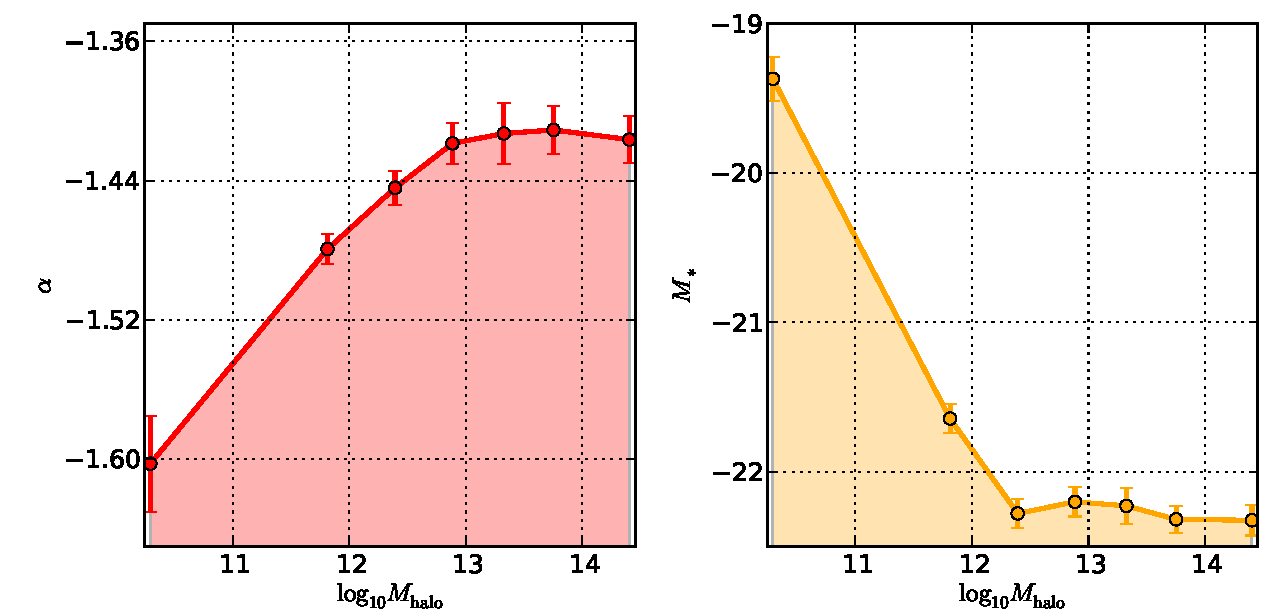
\includegraphics[width=\linewidth]{evolSchechterGuo}}
    \end{minipage}
    \begin{minipage}{\linewidth}
    \centering
    \subfloat[For a double Schechter distribution]{
    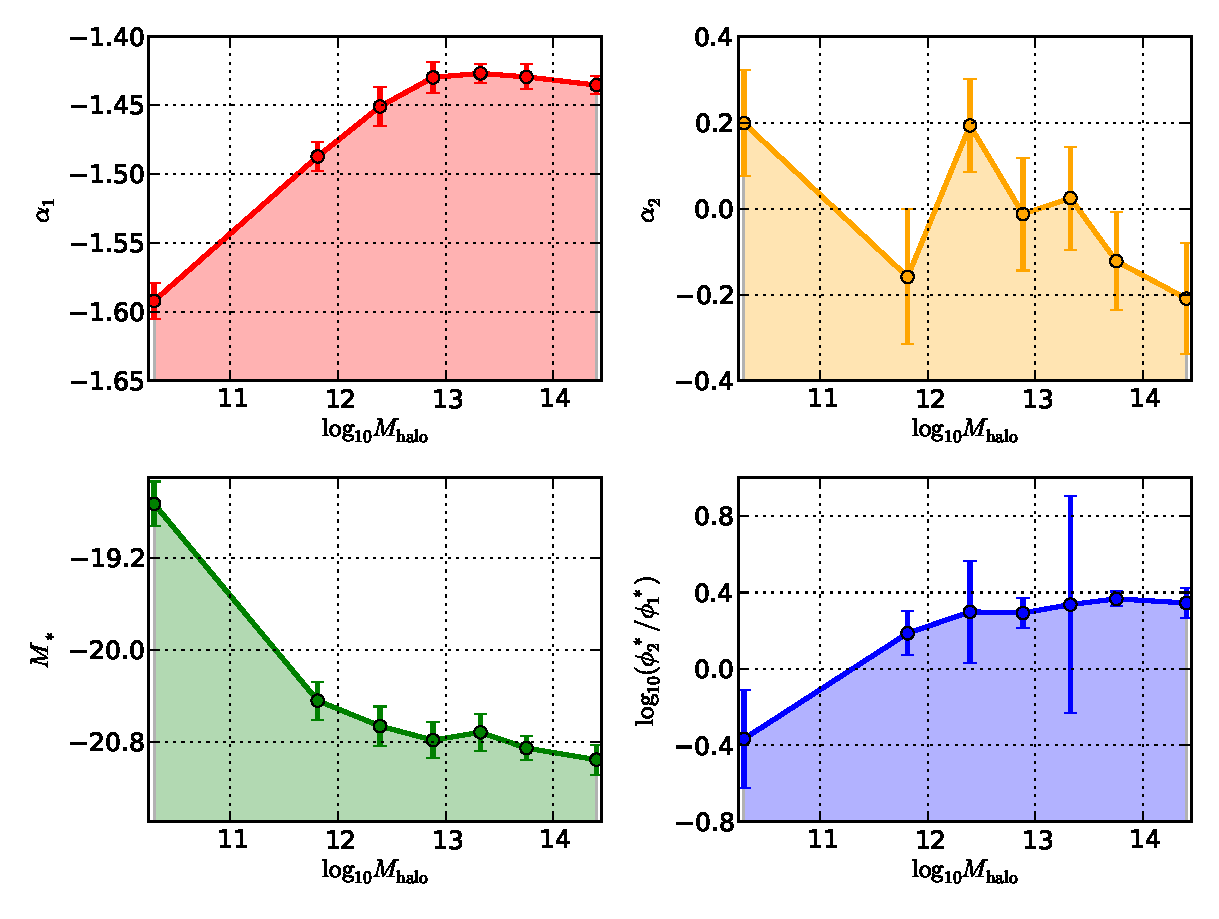
\includegraphics[width=\linewidth]{evolDblSchechterGuo}}
    \end{minipage}
    \caption{\footnotesize{}Modulation of the parameters of both Schechter and double Schechter luminosity distributions with
    the halo mass.}
\label{fig:modsch}
\end{figure*}
The resulting fit of the probability density function is shown for the double Schechter in the figure (\ref{fig:fitguodblsch}).

As we expect, we can see some physics process putted in the SAM in this figure.\com{To detail.}

Therefore, \com{Verify Cependant$\rightarrow$Therefore.}, we don't see a particular modulation, \textit{i.e.} a functional form to
use for each parameter of the DS.\@ So we have decided to use polynomials functions to adjust this modulation. For a given parameter
$\theta_i$ we write:
\begin{eq}
    \theta_i\pg{M}\pd=\sum_{j=0}^N{a_{ij}{M^j}}
\end{eq}
where $N$ is the order of the polynomial.

We now integrate this form of parametrization of the parameters of the DS into the minimization of the likelihood using directly
the halo masses of the galaxies.

But it doesn't work!!!\com{Some blabla!}

\fsss{Flux limited sample}

Working with a flux limited sample, it's like having gaps into the set of galaxies. But we know why we are missing this galaxies: we
can't see them at a given distance. Determining the luminosity limit which we can see at redshift $z$ can be done analytically. So
for that we use the STY method.\com{Put Bibtex of STY and description related to this.} We need to modify the probability density
used in the likelihood to take into account missing data. The procedure is the following: in order to estimate the likelihood, we
have to calculate the probability density for a galaxy $i$ at the redshift $z_i$ of having a magnitude between $M_i$ and $M_i+\dd{M_i}$.
The probability that a galaxy have a magnitude $\mathcal{M}$ superior to $M$ is given by:
\begin{eq}\label{eq:cumprobfluxlim}
    P\pg\mathcal{M}>M|z\pd=\cfrac{\int_{-\infty}^M{\phi\pg{M'}\pd\rho\pg{z}\pd{f\pg{M'}\pd}\dd{M'}}}
    {\int_{-\infty}^{\infty}{\phi\pg{M'}\pd\rho\pg{z}\pd{f\pg{M'}\pd}\dd{M'}}}
\end{eq}
where $f$ is the completeness function and $\rho\pg{z}\pd$ is the redshift distribution. We can express it like this because the
number of galaxies at a given redshift $z$ with a given magnitude $M$ is $\dd{N}=\phi\pg{M}\pd\dd{M}$ in a given volume. So to avoid
the volume dependence, we multiply by the number of galaxies in a given volume $\rho\pg{z}\pd=\dd{N}/\dd{V}$. So the number of
galaxies with a magnitude between $M$ and $M+\dd{M}$ is $\dd^2{N}=\phi\pg{M}\pd\rho\pg{z}\pd\dd{M}\dd{V}$. But with the problem of
the completeness, we can see just galaxies with a certain magnitude defined by $f$ so $\dd^2{N}=\phi\pg{M}\pd\rho\pg{z}\pd
f\pg{M}\pd\dd{M}\dd{V}$. The probability (\ref{eq:cumprobfluxlim}) results from this. Calculating the probability density is straightforward
because we have:
\begin{eq}
    P\pg\mathcal{M}>M|z\pd=\int_{-\infty}^M{p\pg{M'|z}\pd}\dd{M'}
\end{eq}
and so:
\begin{eq}
    p\pg{M|z}\pd=\ddp{P\pg\mathcal{M}>M|z\pd}{M}
\end{eq}
Finally:
\begin{eq}
    p\pg{M_i|z_i}\pd=\dfrac{\phi\pg{M_i}\pd}{\int_{M_{\mathrm{bright}}\pg{z_i}\pd}^{M_{\mathrm{faint}}\pg{z_i}\pd}
    {\phi\pg{M'}\pd\dd{M'}}}
\end{eq}
and this defines the new likelihood in the case of a flux limited sample.

We apply this to the incomplete sample generated with the mock algorithm we have created. Firstly, we have tried to recover the
parameters in the mock with the apparent magnitudes calculated applying a ``K-decorrection''. The results are very bad. Parameters
can't be recovered correctly and with the two models chosen (simple Schechter and DS). We don't have the same estimations as in the
complete sample, although the flux limited sample is the same as the complete sample but ``truncated''. It's not clear why this
parameters can't be found. The procedure isn't in cause, but it's possible that the data are the problem. We think that our method
for estimating the K-decorrection have some troubles when the redshift is higher than \num{0.2}.

For verifying this assumption, we have made more simple flux limited samples. We know how to generate random variables following a
Schechter distribution and a DS distribution two. We have placed galaxies in a homogeneous universe, up to few hundred Mpc. We have
assigned redshifts to this galaxies according to their distances $D$ using simply $z=v/c={H_0}{D}/c$. We apply a Schechter
distribution to the galaxies generated, without taking clusters effects into account. Calculating apparent magnitudes is done
subtracting the distance modulus using galaxies redshifts. We have done the same applying a DS.\@ Results are the followings:
\begin{itemize}
    \item We are enable to recover the Schechter parameters used to generate the distribution in the flux limited sample. When
    data are perfect like in this situation, there are no troubles.
    \item Using a DS distribution, we have more difficulties in finding those parameters used to generate the flux limited
    sample. The slopes of both the low galaxies and brighter galaxies aren't near the true values.
\end{itemize}
We think that the number of low galaxies in the flux limited sample isn't not sufficient to well constrain the slopes in the DS.\@ As
a result, the maximum likelihood can't find real parameters. It's like a degeneracy is present and the algorithm can't decide to the
true parameters.
\begin{figure}[htb]
    \centering
    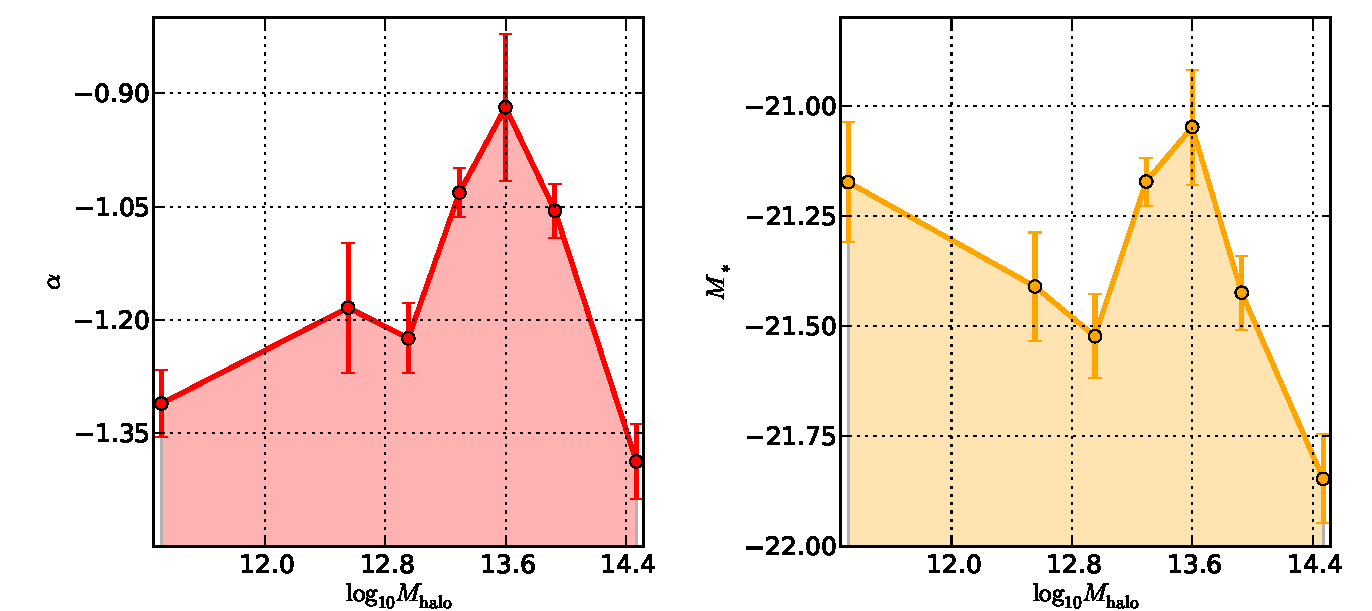
\includegraphics[width=0.8\linewidth]{evolSchechterMock}
    \caption{\footnotesize{}Modulation of the parameters for a Schechter distribution with the halo mass in a mock catalogue
    constructed with the galaxy catalogue from the Guo2010a, without taking a K-decorrection for apparent magnitudes of
    galaxies.}
\label{fig:parammock}
\end{figure}

So, it's a clue that the K-decorrection isn't good at high redshift and underestimate the number of galaxies when we apply a flux
limit using apparent magnitudes. We have made an other mock catalogue without this K-decorrection in order to show that is the real
problem. We have extended too the upper magnitude limit of galaxies in the sample in order to improve the number of low galaxies to
estimate better slopes in the case of the DS.\@ The former limit was \num{-15} in $r$ band magnitude and now we go to \num{-12}. So we
expect that the number of low luminosity galaxies increases and improves the parametrization. All results hereafter and before are
for this new limit.

Unfortunately, the increasing number of low mass galaxies and taking no K-decorrection doesn't improve the estimation of the
parameters. Results are shown in figure (\ref{fig:parammock}).
\begin{figure}[htb]
    \centering
    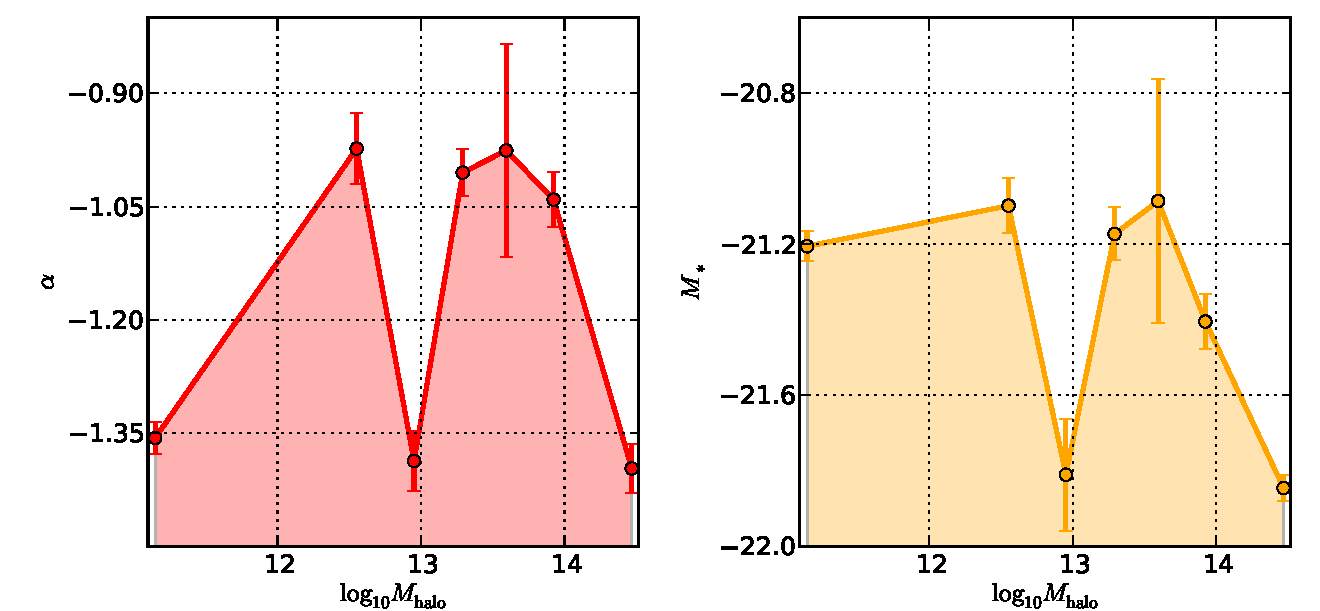
\includegraphics[width=0.8\linewidth]{evolSchechterMockNoBorder}
    \caption{\footnotesize{}Modulation of the parameters for a Schechter distribution with the halo mass in a mock catalogue
    constructed with the galaxy catalogue from the Guo2010a, without taking a K-decorrection for apparent magnitudes of
    galaxies and removing galaxies in groups that are closer to the border of cube simulation on the mock's cube.}
\label{fig:parammocknoborder}
\end{figure}

We can see that the modulation of this parameters with the halo mass isn't the same as in the figure (\ref{fig:modsch}) for the
Schechter distribution. It's not very clear why when we construct the mock catalogue, we can't recover the same parameters as for
the data used to build this mock catalogue. It's maybe a problem of spatial truncation of data in flux and redshift that may cause
some variations on the intrinsic LF of the data from the galaxy catalogue used for the mock catalogue. The mock catalogue have a
problem: periodic conditions in the box used in order to build this mock can move away from each other galaxies belonging to the
same group. So in groups of a certain halo mass, we have more missing data than expected and the estimation of parameters is
affected too. To see if this assumption is correct, we have removed from the sample of galaxies in the mock catalogue these ones
that are in groups too close to the border of the box in the mock catalogue. The modulation is shown on the figure
(\ref{fig:parammocknoborder}).

We can't find parameters as in the galaxy catalogue from \citet{Guo+11} both with modulation of the halo mass and for global data.
The behaviour is the same as the latter situation.
\begin{figure}[htb]
    \centering
    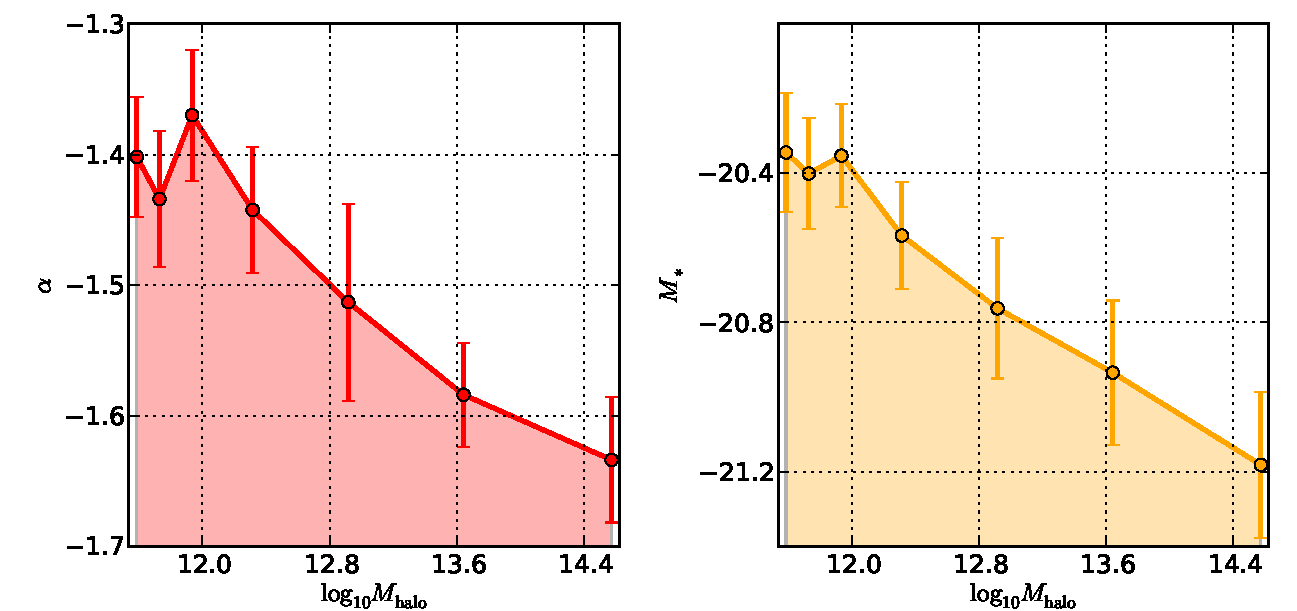
\includegraphics[width=0.8\linewidth]{evolSchechterLinGalPop}
    \caption{\footnotesize{}Modulation of the parameters for a Schechter distribution with the halo mass in the sample of galaxy
    constructed using a HOD model, and imposing a linear evolution of the parameters with halo mass. We have imposed that
    $\alpha$ goes from \num{-1.2} to \num{-1.7} and $M_*$ from \num{-19.5} and \num{-21.5} between the extreme halo mass of the
    simulation.}
\label{fig:paramschlin}
\end{figure}

The last test to understand why we can't find the same parameters is described in what follows. We have used the algorithm described
in the appendix \com{add the description in the appendix to generate a galaxy population from a simulation} in order to create a
sample of galaxy following a NFW profil in halos, with a velocity dispersion calculated using the \citet{ML05} model for the
anisotropy factor. Galaxy luminosities in the halo are generated in order to have a linear modulation of the parameters of a
Schechter distribution with the halo mass. We imposed this modulation in the data of the galaxy sample generated with the HOD model
of~\cite{Zehavi+11}. The magnitude sample has $\num{-23}<M_r<\num{-12}$. The result of this modulation in the complete sample is
shown in figure (\ref{fig:paramschlin}).

We now construct an other mock catalogue using this galaxy sample in order to see what happened when we fix the modulation in the
parameters with the halo mass in a flux limited sample.
Results are shown on the figure (\ref{fig:paramschlin})

The mock catalogue we have created goes to a redshift of \num{0.1} while the mock with the galaxy sample from \citet{Guo+11} is
limited to a redshift of \num{0.3}.
The modulation of the parameters we have imposed in the galaxy sample is well recovered. In the case of $M_*$, the estimation
is always good, same with a DS.\@ But there are more uncertainties in finding the slope of the LF with both Schechter and DS.\@ Slopes
are less constrained by the data when with have a flux limited sample.
\begin{figure}[htb]
    \centering
    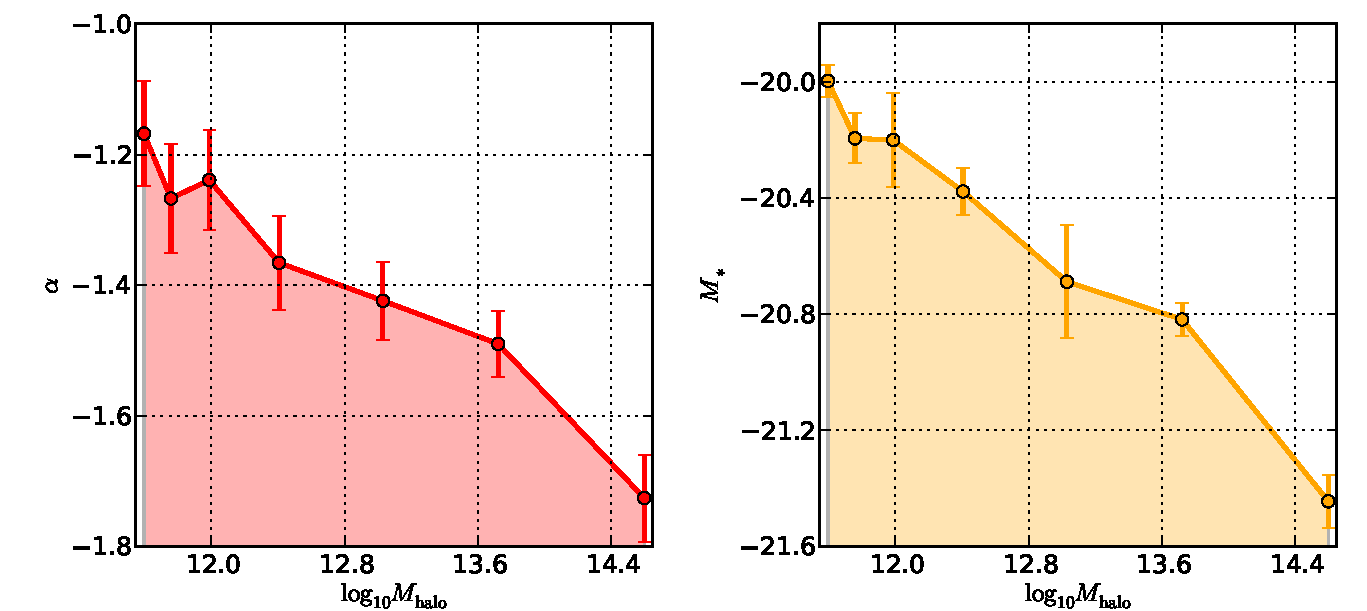
\includegraphics[width=0.8\linewidth]{evolSchechterLinMockGalPop}
    \caption{\footnotesize{}Modulation of the parameters for a Schechter distribution with the halo mass in the mock catalogue
    constructed as described in the previous figure. Parameters are recovered with a given uncertainties.}
\label{fig:paramschlinmock}
\end{figure}

%\scriptsize{\cbleu{\bibliography{ref}}}
%\normalsize

%\appendix

% adding files for the appendix
\bartchapterimage{heic0911c.jpg}
\chapter{Density profiles}
\label{cha:profiles}
\bartthumb{heic0911c.png}

\section{Introduction}

In this chapter, we provide details on the computation of the density profiles
and their derived quantities. We define here the different normalizations used
along the thesis for some popular density profiles.

\subsection{Definitions}

The number of galaxies in a sphere of radius $r$ with a density profile in
number $\nu(r)$ is the case of a spherical symmetry:
%
\begin{equation}
    N\left(r\right)=\int_0^r4\pi {r'}^2 \nu(r')\dd{r'}
\end{equation}

To start, we define some dimensionless functions to facilitate the
computations.
%
\begin{eqnarray}
    N\left(r\right)&=N\left(a\right){\widetilde{N}\left(r/a\right)}\nonumber\\
    \nu\left(r\right)&=
        \cfrac{N\left(a\right)}{4\pi{a^3}}
        \,\widetilde\nu\left(r/a\right)
\end{eqnarray}
%
with $a$ the radius at which the logarithmic slope of the density profile is
equal to $-2$. We also define the same relations for a
virial normalization.
%
\begin{eqnarray}
    N\left(r\right)&={N_v}\,{\widehat{N}\left(r/\rvir\right)}\nonumber\\
    \nu\left(r\right)&=
        \cfrac{N_v}{4\pi\rvir^3}\,\widehat\nu\left(r/\rvir\right)
\end{eqnarray}

We also define the concentration $c$ as the ratio between the virial radius
$\rvir$ and the radius $a$, i.e.\ $c=\rvir/a$. We define $\rvir=r_{200}$ for
simplicity.

\section{Density profiles}
\label{sec:density_profiles}

\subsection{\citet{NFW+97}}

The NFW density profile is:
%
\begin{equation}
    \nu \left(r\right) = \cfrac{\nu_0}{r {\left(r+a\right)}^2}
\end{equation}
%
with $\nu_0$ a constant density.

We can write by integrating previous relations with $\int_0^1
x^2\widetilde\nu\dd x=\int_0^1 x^2\widehat\nu\dd x$  and searching for the
constant $\nu_0$:
%
\begin{equation}
    \widetilde\nu\left(x\right)=\cfrac{1}{\ln2-1/2}
        \quad\cfrac{1}{x{\left(1+x\right)}^2}
\end{equation}
%
\begin{equation}
    \widetilde{N}\left(x\right)=\cfrac{1}{\ln2-1/2}
        \quad\left(\ln\left(1+x\right)-\cfrac{x}{x+1}\right)
\end{equation}
%
\begin{equation}
    \widehat\nu\left(x\right)=
        \cfrac{1}{\ln\left(1+c\right)-c/ \left(1+c\right)}
        \quad\cfrac{1}{x{\left(1/c+x\right)}^2}
\end{equation}
%
\begin{equation}
    \widehat{N}\left(x\right)=
        \cfrac{1}{\ln \left(1+c\right)-c/ \left(1+c\right)}
        \quad\left(\ln\left(1+xc\right)-\cfrac{xc}{xc+1}\right)
\end{equation}

\subsection{Einasto}
\label{sub:einasto}

For an Einasto density profile:
\begin{equation}
    \nu \left(r\right) = \nu_0 \exp
    \left[- {\left(\cfrac{r}{b}\right)}^{1/m}\right]
\end{equation}

Writing the definition of the $a$ radius with this density profile, we have:
%
\begin{equation}
    {\left(\cfrac{1}{b}\right)}^{1/m} = 2m{\left(\cfrac{1}{a}\right)}^{1/m}
\end{equation}
%
leading to the following normalizations:
%
\begin{equation}
    \widetilde\nu \left(x\right) = \cfrac{{\left(2m\right)}^{3m}}{m\gamma
    \left(3m, 2m\right)} \exp \left(-2mx^{1/m}\right)
\end{equation}
%
\begin{equation}
    \widetilde{N} \left(x\right) = \cfrac{\gamma \left(3m, 2m
    x^{1/m}\right)}{\gamma \left(3m, 2m\right)}
\end{equation}
%
\begin{equation}
    \widehat\nu \left(x\right) = \cfrac{{\left(2m\right)}^{3m}}{m\gamma
    \left(3m, 2m c^{1/m}\right)} \exp \left(-2m{\left(xc\right)}^{1/m}\right)
\end{equation}
%
\begin{equation}
    \widehat{N} \left(x\right) = \cfrac{\gamma \left(3m, 2m
        {\left(xc\right)}^{1/m}\right)}{\gamma \left(3m, 2m c^{1/m}\right)}
\end{equation}

\subsection{Generalized NFW}
\label{sub:generalized_nfw}

If any previous density profiles isn't sufficient to describe the distribution
of dark matter particles or galaxies inside the halos, a solution is possibly
to fit a generalized NFW profile, whose the density is:
%
\begin{equation}
    \nu \left(r\right) =
    \cfrac{\nu_0}{r^\alpha{\left(r+a\right)}^{\beta-\alpha}}
\end{equation}

In this case:
%
\begin{equation}
    \widetilde{N} \left(x\right) = \cfrac{%
        \mathcal{B}_{-x} \left(3-\alpha, 1+\alpha-\beta\right)}
    {\mathcal{B}_{-1} \left(3-\alpha, 1+\alpha-\beta\right)}
\end{equation}
%
therefore:
%
\begin{equation}
    \widetilde\nu \left(x\right) = \cfrac{1}
    {{\left(-1\right)}^{\alpha+1}
        \mathcal{B}_{-1} \left(3-\alpha, 1+\alpha-\beta\right)}
    \quad\cfrac{1}
    {x^\alpha {\left(1+x\right)}^{\beta-\alpha}}
\end{equation}
%
For the virial normalization:
%
\begin{equation}
    \widehat{N} \left(x\right) = \cfrac{%
        \mathcal{B}_{-xc} \left(3-\alpha, 1+\alpha-\beta\right)}
    {\mathcal{B}_{-c} \left(3-\alpha, 1+\alpha-\beta\right)}
\end{equation}
%
\begin{equation}
    \widehat\nu \left(x\right) = \cfrac{1}
    {{\left(-1\right)}^{\alpha+1}
        \mathcal{B}_{-c} \left(3-\alpha, 1+\alpha-\beta\right)}
    \quad\cfrac{1}
    {{\left(xc\right)}^\alpha {\left(1+xc\right)}^{\beta-\alpha}}
\end{equation}
%
where $\mathcal{B}$ is the function defined as:
%
\begin{equation}
    \mathcal{B} \left(a, b\right) =
    \cfrac{\Gamma \left(a\right) \Gamma \left(b\right)}
    {\Gamma \left(a+b\right)} =
    \int_0^1 t^{a-1} {\left(1+t\right)}^{b-1} \dd t
\end{equation}
%
and its incomplete version is:
%
\begin{equation}
    \mathcal{B}_z \left(a, b\right) =
    \int_0^z t^{a-1} {\left(1+t\right)}^{b-1} \dd t
\end{equation}

\section{Radial velocity dispersion}
\label{sec:radial_velocity_dispersion}

Galaxies in groups (and their associated dark matter halos) are assumed to be a
system of particles only submitted to the gravitation. Neglecting mergers and
other physical processes inside galaxy groups, the number of galaxies doesn't
evolve in phase space, and the distribution function is constant along the
evolution of the system. In this case, we can use the collisionless Boltzmann
equation to extract dynamical properties of galaxy groups.

The Jeans equation is the first velocity momentum of the Boltzmann equation. In a
spherical symmetry, assuming stationarity, the Jeans equation is:
%
\begin{equation}
    \label{eq:jeans}
    \ddp{\left[\nu(r)\sigma_r^2(r)\right]}{r} +
    \cfrac{2\mybeta}{r}\left[\nu(r)\sigma_r^2(r)\right]=
    -\nu(r)\cfrac{GM(r)}{r^2}
\end{equation}
%
where $\beta \left(r\right)$ is the radial profile of velocity anisotropy
$\beta = 1 - \sigma_\theta^2/\sigma_r^2$.

We can compute the radial velocity dispersion using \bartrefequation{jeans} for
a spherical system at equilibrium. The solution to this equation is given by:
%
\begin{equation}
    \myprofil\sigma_r^2(r)=
    \int_r^\infty K_r(r,s)\nu(s)\cfrac{GM(s)}{s^2}\,\dd{s}
\end{equation}
%
with $K_r(r,s)$ the kernel of the integral defined as:
%
\begin{equation}
    K_r(r,s)=\exp\left[2\int_r^s\mybeta\cfrac{\dd{t}}{t}\right]
\end{equation}

There are two ways of normalizing the radial velocity dispersion according to
the normalization used for the density and mass profiles. We show it for the
virial normalization for illustration:
%
\begin{equation}
    \label{eq:sigma_norm}
    \widehat\sigma_r^2(x)= \cfrac{1}{\widehat\nu \left(x\right)}
    \int_x^\infty K_r(x,s)\widehat\nu(s)\cfrac{\widehat{M}(s)}{s^2}\,\dd s
\end{equation}
%
with:
%
\begin{equation}
    \sigma_r^2(r) = \cfrac{GM_v}{\rvir}\,\widehat\sigma_r^2(r/\rvir)
\end{equation}

We are interested only in the NFW profile in the thesis, since it is accurate
enough to adjust the model. If we want an analytical form for $\sigma_r
\left(r\right)$, we need to choose a model for the anisotropy profile $\beta
\left(r\right)$. We provide here some expressions of the radial velocity
dispersion, assuming the NFW density profile, for a useful anisotropy model.

\subsection{\citet{ML+05}}
\label{sub:ml05}

This model is of the form:
%
\begin{equation}
    \beta \left(r\right) = \undemi\cfrac{r}{r+b}
\end{equation}
%
where $b$ is a characteristic radius of the model. Introducing this expression
in \bartrefequation{sigma_norm}, we obtain:
%
\begin{align}
    \widetilde\sigma_r^2(x)=&
        -\frac{1}{3 x (1+r x)
        {(-1+\ln\left(4\right))}^2}2
        \left(-\frac{1}{2}+\ln\left(2\right)\right)\nonumber\\
    &\left(x \left(3+x \left(\pi ^2 (-3+2 r)
        {(1+x)}^2-3 (-9+5 r-7 x+4 r x)
        \right)\right.\vphantom{\ln\left(1+\frac{1}{x}\right)}\right.
        \nonumber\\
    &\left.-3 x^3 \ln\left(1+\frac{1}{x}\right)+3 x (1+2 x)
        \ln\left(x\right)\right)\nonumber\\
    & -3 (1+2 x (-1-2 x (2+x)+r (1+x) (1+2 x)))
        \ln\left(1+x\right)+3 (-3+2 r) {\left(x+x^2\right)}^2
        \ln{\left(1+x\right)}^2\nonumber\\
    & \left.+6 (-3+2 r) x^2 {(1+x)}^2
        Li_2\left(-x\right)\vphantom{\ln\left(1+\frac{1}{x}\right)}\right)
        \nonumber\\
\end{align}
\begin{align}
    \widehat\sigma_r^2(x)=&
        \frac{1}{6 x (1+r x) \left(-1+\frac{1}{1+c}+\ln c\right)}
        \left(c x \left(-3+x \left(3 c \left(-9+\pi ^2\right)+
        \left(15-2 \pi ^2\right) r\right.\right.
        \vphantom{{(1+c x)}^2}\right.\\
    &\left. -4 c \left(-3+\pi ^2\right) r x+
        3 c^3 \pi ^2 x^2+c^2 x \left(-21+\pi ^2 (6-2 r x)\right)\right)\\
    & \left.+6 c^3 x^3 {\rm arccoth} \left(1+2 c x\right)-
        3 c x (1+2 c x) \ln\left(c x\right)\right)\\
    &+3(1+2 x (r+c (-1+x (-4 c+3 r+2 c (-c+r) x))))
        \ln\left(1+c x\right)\\
    &\left.+3c(3 c-2 r) x^2 {(1+c x)}^2 {\left(\ln\left(1+c x\right)\right)}^2+
    6 c (3 c-2 r) x^2 {(1+c x)}^2 \mathrm{Li_2}\left(-c x\right)\right)\\
\end{align}

\section{Line of sight velocity variance}

We will compute in this section the line of sight velocity dispersion of
galaxies in a general spherical density profile, and then compute it
specifically for an NFW profile. This is useful to make cuts at
$\pm\kappa\sigma_\mathrm{LOS} \left(R\right)$ in the \pps{}.

By definition, the variance is the mean of the squared quantity. We use a
general density profile which is invariant under rotations $\nu{(r)}$. In our
case, we make this mean on the line of sight, so:
%
\begin{equation}
    \sigma_\mathrm{LOS}^2\left({R}\right)=
    \cfrac{\int_{-\infty}^{\infty}{v_\mathrm{LOS}^2}\nu{(r)}\,\dd{z}}
    {\int_{-\infty}^{\infty}\nu{(r)}\,\dd{z}}
\end{equation}
%
But in the group, $r^2=R^2+z^2$ so:
%
\begin{equation}
    \sigma_\mathrm{LOS}^2\left({R}\right)=
    \cfrac{2\int_{R}^{r_{\max}}{v_\mathrm{LOS}^2}
    \cfrac{\nu{(r)}{r}}{\sqrt{r^2-R^2}}\,\dd{r}}
    {2\int_{R}^{r_{\max}}\cfrac{\nu{(r)}{r}}{\sqrt{r^2-R^2}}\,\dd{r}}
\end{equation}
%
The denominator is by definition the projected density surface along the line
of sight and we denote it
%
\begin{equation}
    \Sigma(R) = 2\int_{R}^{r_{\max}}\cfrac{\nu{(r)}{r}}{\sqrt{r^2-R^2}}\,\dd{r}
\end{equation}
%
Normally the integration is for $r_{\max}\rightarrow\infty$ but in our case we
want to restrict to a limited region in the group (to the virial sphere
precisely).

In the same coordinate system as previously, the line of sight velocity can be
expressed in spherical coordinates as:
%
\begin{equation}
    v_{\mathrm{LOS}} = v_r \cos\theta - v_\theta \sin\theta
\end{equation}
%
We suppose that we are at the equilibrium and so that there is no flow in the
group in consequence we can neglect means of velocities. In terms of velocity
variance we have now:
%
\begin{equation}
    \mysigma\mysiglos = 2\int_R^{r_{\max}}
    \left({\sigma_r^2(r)\cos^2\theta+\sigma_\theta^2\sin^2\theta}\right)
    \cfrac{\nu{(r)}{r}}{\sqrt{r^2-R^2}}\,\dd{r}
\end{equation}
%
If we want to use the anisotropy parameter
$\mybeta=1-\sigma_\theta^2(r)/\sigma_r^2(r)$ in case of sphericity, we can
write:
%
\begin{equation}
    \mysigma\mysiglos = 2\int_R^{r_{\max}}
    \left({1-\mybeta\cfrac{R^2}{r^2}}\right)
    \cfrac{\nu{(r)}{\sigma_r^2(r)}{r}}{\sqrt{r^2-R^2}}\,\dd{r}
\end{equation}

We can compute the radial velocity dispersion using the Jeans equation for a
spherical system at equilibrium.

\subsection{\citet{ML+05} anisotropy}

With the decomposition of the integral over the domain of integration, we can
write:
%
\begin{align}
    \Sigma{(R)}{\sigma_\mathrm{LOS}}^2{(R)}=&
        2\int_R^{r_v}{\cfrac{\left({s+a}\right)}{s^2}{\nu(s)}{G}{M(s)}}{\dd{s}}
        \nonumber\\
    &\times
        \left(\int_R^s{\left(\cfrac{r}{r+a}-\undemi
        {\left(\cfrac{R}{r+a}\right)}^2\right)
        \cfrac{1}{\sqrt{r^2-R^2}}\dd{r}}\right)\nonumber\\
    &+2\int_{r_v}^{\infty}
        \cfrac{\left({s+a}\right)}{s^2}\nu(s){G}{M(s)}\dd{s}\nonumber\\
    &\times
        \left(\int_R^{r_v}
            \left(\cfrac{r}{r+a}-\undemi{\left(\cfrac{R}{r+a}\right)}^2\right)
            \cfrac{1}{\sqrt{r^2-R^2}}\dd{r}\right)
\end{align}
%
where we are setting $r_{\max}$ to $r_v$. So now we can write:
%
\begin{align}
    {\sigma_\mathrm{LOS}}^2{(R)}=&{v_v}^2\cfrac{c/2}{\widetilde{M}{(c)}\widetilde{\Sigma}{(R/a,c)}}\nonumber\\
    &\times\left(\int_{R/a}^c{{K}\left({x\cfrac{a}{R},\cfrac{a}{R}}\right)}\widetilde{\nu}{(x)}
    \cfrac{\widetilde{M}{(x)}}{x}\dd{x}+I\left({c\cfrac{a}{R},\cfrac{a}{R}}\right){J(c)}\right)
\end{align}
%
\begin{equation}
    I(u,u_a)=\left\{\begin{array}{lr}
        -u_a{\rm{sign}}(u_a-1)\cfrac{{u_a}^2-1/2}{|{u_a}^2-1|^{3/2}}{C^{-1}\left(\cfrac{1+u{u_a}}{u+u_a}\right)}&\\
        \hspace{5em}+{\rm{acosh}}{u}+\cfrac{1/2}{u_a+u}\cfrac{\sqrt{u^2-1}}{{u_a}^2-1},&{u_a}\neq1\\
        {\rm{acosh}}{u}-\sqrt{\cfrac{u-1}{u+1}}\left(\cfrac{8+7u}{6(1+u)}\right),&{u_a}=1\\
    \end{array}\right.
\end{equation}
%
with:
%
\begin{equation}
    K(u,u_a)=\left({1+\frac{u_a}{u}}\right){I(u,u_a)}
\end{equation}
%
and:
%
\begin{equation}
    C^{-1}(X)=\left\{\begin{array}{lr}
        {\rm{acosh}}{X}&u_a>1\\
        {\rm{acos}}{X}&u_a<1\\
    \end{array}\right.
\end{equation}
%
We also have an other integral:
%
\begin{equation}
    J(y)=\int_y^{\infty}\frac{x+1}{x^2}\widetilde{\nu}{(x)}\widetilde{M}{(x)}\dd{x}
\end{equation}
%
In the case of an NFW profile, this can be expressed in an analytical way:
%
\begin{align*}
    J(y)=&
        \frac{2}{3{y^2}(1+y){\left(\ln{4}-1\right)}^2}
        \left(y\left(-3+y\left(-9+\pi^2\left(1+y\right)\right)\right)\right.\\
    &+3{y^3}\ln\left(1+\frac{1}{y}\right)+3\ln\left(1+y\right)
            \left(1-y+y^2\left(1+y\right)\ln\left(1+y\right)\right)\\
    &\left.-3{y^2}\ln\left({y}\left(1+y\right)\right)+6{y^2}
        \left(1+y\right){\dilog{-y}}\right)\\
\end{align*}
%
where the dilogarithm function is defined in our case as:
%
\begin{equation}
    \dilog{z}=-\int_0^1\cfrac{\ln{(1-zt)}}{z}\,\dd{t}
\end{equation}

For the NFW model, \citet{MBM+10} provide the expression of
$\widetilde{\Sigma}$:
%
\begin{multline}
    \widetilde{\Sigma}(X,c)=\cfrac{1}{2\ln2-1}\int_X^c\cfrac{\dd{x}}{{(1+x)}^2\sqrt{x^2-X^2}}\\
    =\cfrac{1}{2\ln2-1}\begin{cases}
        \cfrac{1}{{(1-X^2)}^{3/2}}
        \cosh^{-1}\left[\cfrac{c+X^2}{(c+1)X}\right]-
        \cfrac{1}{(c+1)}\cfrac{\sqrt{c^2-X^2}}{1-X^2} &\text{if } 0<X<1 \\
    \cfrac{\sqrt{c^2-1}(c+2)}{3{(c+1)}^2} &\text{if } X=1<c\\
    \cfrac{1}{(c+1)}\cfrac{\sqrt{c^2-X^2}}{X^2-1}-
    \cfrac{1}{{(X^2-1)}^{3/2}}
    \cos^{-1}\left[\cfrac{c+X^2}{(c+1)X}\right] &\text{if } 1<X<c\\
    0 &\text{if } X=0\,\text{or}\,X>c
    \end{cases}
\end{multline}

% vim: set tw=79 : set concealcursor=

%
\chapter{Line of sight velocity variance}

\newcommand{\mybeta}{%
\beta(r)%
}
\newcommand{\mysigma}{%
\Sigma(r)%
}
\newcommand{\mysiglos}{%
\sigma_{\mathrm{LOS}}^2(R)%
}
\newcommand{\myprofil}{%
\nu(r)%
}

\section{Introduction}

We will compute in this section the line of sight velocity dispersion
of galaxies in a general spherical density profile, and then compute it
specifically for an NFW profile.

This useful to make cuts at some sigma in the velocity profile to check
where is the most important part of a group.

\section{Calculus}

By definition, the variance is the mean of the squared quantity under the
assumption of a distribution function.
We use a general density profile which is invariant under rotations $\nu{(r)}$.
In our case, we make this mean on the line of sight, so:
\[
\sigma_{LOS}^2\pg{R}\pd=\cfrac{\int_{-\infty}^{\infty}{v_{LOS}^2}\nu{(r)}\dd{z}}
{\int_{-\infty}^{\infty}\nu{(r)}\dd{z}}
\]
But in the group $r^2=R^2+z^2$ so:
\[
\sigma_{LOS}^2\pg{R}\pd=\cfrac{2\int_{R}^{r_{\mathrm{max}}}{v_{LOS}^2}\cfrac{\nu{(r)}{r}}{\sqrt{r^2-R^2}}\dd{r}}
{2\int_{R}^{r_{\mathrm{max}}}\cfrac{\nu{(r)}{r}}{\sqrt{r^2-R^2}}\dd{r}}
\]
The denominator is by definition the projected density surface along the line of sight
and we denote it
\[
\Sigma(R) = 2\int_{R}^{r_{\mathrm{max}}}\cfrac{\nu{(r)}{r}}{\sqrt{r^2-R^2}}\dd{r}
\]
Normally the integration is for $r_{\mathrm{max}}\rightarrow\infty$ but in our case
we want to restrict to a limited region in the group (to virial sphere precisely).

In the same coordinate system as previously, the line of sight velocity can be expressed
in spherical coordinates as:
\[
v_{\mathrm{LOS}} = v_r \cos\theta - v_\theta \sin\theta
\]
We suppose that we are at the equilibrium and so that there is
no flow in the group in consequence we can neglect means of velocities.
In terms of velocity variance we have now:
\[
\mysigma\mysiglos = 2\int_R^{r_{\mathrm{max}}}
\pg{\sigma_r^2(r)\cos^2\theta+\sigma_\theta^2\sin^2\theta}\pd
\cfrac{\nu{(r)}{r}}{\sqrt{r^2-R^2}}\dd{r}
\]
If we want to use the anisotropy parameter $\mybeta=1-\sigma_\theta^2(r)/\sigma_r^2(r)$
in case of sphericity\postit{Check word sphericity!}{5}, we can write:
\[
\mysigma\mysiglos = 2\int_R^{r_{\mathrm{max}}}
\pg{1-\mybeta\cfrac{R^2}{r^2}}\pd
\cfrac{\nu{(r)}{\sigma_r^2(r)}{r}}{\sqrt{r^2-R^2}}\dd{r}
\]

We can compute the radial velocity dispersion using the Jeans equation
for a spherical system at equilibrium.
\[
\ddp{\pg\nu(r)\sigma_r^2(r)\pd}{r} + \cfrac{2\mybeta}{r}\pg\nu(r)\sigma_r^2(r)\pd=
-\nu(r)\cfrac{GM(r)}{r^2}
\]
The solution to this equation is given by:
\[
\myprofil\sigma_r^2(r)=\int_r^{r_{\mathrm{max}}}K_r(r,s)\nu(s)\cfrac{GM(s)}{s^2}\dd{s}
\]
with $K_r(r,s)$ the kernel of the integral defined as:
\[
K_r(r,s)=\exp\left[2\int_r^s\mybeta\cfrac{\dd{t}}{t}\right]
\]
\begin{figure}[H]
    \centering
    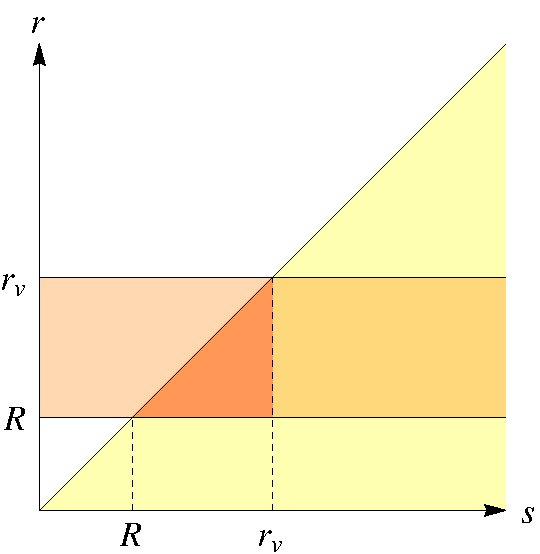
\includegraphics[width=0.5\linewidth]{domint}
    \caption{\footnotesize{}Integration domain for the line of sight radial dispersion.}
    \label{fig:domint}
\end{figure}

\subsection{Supposing \citet{ML05} anisotropy}
With the decomposition of the integral over the domain of integration, we can write
\begin{eqnarray}
    &&\Sigma{(R)}{\sigma_{LOS}}^2{(R)}=2\int_R^{r_v}{\frac{\pg{s+a}\pd}{s^2}{\nu(s)}{G}{M(s)}}{\dd{s}}\nonumber\\
    &\times&\pg\int_R^s{\pg\frac{r}{r+a}-\undemi\pg\frac{R}{r+a}\pd^2\pd\frac{1}{\sqrt{r^2-R^2}}\dd{r}}\pd\nonumber\\
    &+&2\int_{r_v}^{\infty}{\frac{\pg{s+a}\pd}{s^2}{\nu(s)}{G}{M(s)}}{\dd{s}}\nonumber\\
    &\times&\pg\int_R^{r_v}{\pg\frac{r}{r+a}-\undemi\pg\frac{R}{r+a}\pd^2\pd\frac{1}{\sqrt{r^2-R^2}}\dd{r}}\pd\nonumber\\
\end{eqnarray}
where we are setting $r_{\mathrm{max}}$ to $r_v$.
So now we can write using the fact that $4a\nu(a)\widetilde{\Sigma}(R/a,c)$:
\begin{eqnarray}
    &&{\sigma_{LOS}}^2{(R)}={v_v}^2\frac{c/2}{\widetilde{M}{(c)}\widetilde{\Sigma}{(R/a,c)}}\nonumber\\
    &\times&\pg\int_{R/a}^c{{K}\pg{x\frac{a}{R},\frac{a}{R}}\pd}\widetilde{\nu}{(x)}
    \frac{\widetilde{M}{(x)}}{x}\dd{x}+I\pg{c\frac{a}{R},\frac{a}{R}}\pd{J(c)}\pd\nonumber\\
\end{eqnarray}
\begin{equation}
    I(u,u_a)=\left\{\begin{array}{lr}
        -u_a{\rm{sign}}(u_a-1)\frac{{u_a}^2-1/2}{|{u_a}^2-1|^{3/2}}{C^{-1}\pg\frac{1+u{u_a}}{u+u_a}\pd}&\\
        \hspace{5em}+{\rm{acosh}}{u}+\frac{1/2}{u_a+u}\frac{\sqrt{u^2-1}}{{u_a}^2-1},&{u_a}\neq1\\
        {\rm{acosh}}{u}-\sqrt{\frac{u-1}{u+1}}\pg\frac{8+7u}{6(1+u)}\pd,&{u_a}=1\\
    \end{array}\right.
\end{equation}
with:
\begin{eq}
        K(u,u_a)=\pg{1+\frac{u_a}{u}}\pd{I(u,u_a)}
\end{eq}
and:
\begin{eq}
    C^{-1}(X)=\left\{\begin{array}{lr}
        {\rm{acosh}}{X}&u_a>1\\
        {\rm{acos}}{X}&u_a<1\\
    \end{array}\right.
\end{eq}
We have too an other integral:
\begin{eq}
        J(y)=\int_y^{\infty}\frac{x+1}{x^2}\widetilde{\nu}{(x)}\widetilde{M}{(x)}\dd{x}
\end{eq}
In the case of an NFW profile, this can be expressed in an analytical way:
\begin{align*}
        J(y)&=\frac{2}{3{y^2}(1+y)\pg\ln{4}-1\pd^2}\pg{y}\pg-3+y\pg-9+\pi^2\pg1+y\pd\pd\pd\right.\\
        &+3{y^3}\ln\pg1+\frac{1}{y}\pd+3\ln\pg1+y\pd\pg1-y+y^2\pg1+y\pd\ln\pg1+y\pd\pd\\
        &\left.-3{y^2}\ln\pg{y}\pg1+y\pd\pd+6{y^2}\pg1+y\pd{\dilog{-y}}\pd\\
\end{align*}
where the dilogarithm function is defined in our case as:
\[
\dilog{z}=-\int_0^1\cfrac{\ln{(1-zt)}}{z}\dd{t}
\]

Still in the case of the NFW profil, in \citet{MBM10} there is the expression of $\widetilde{\Sigma}$:
\begin{multline}
    \widetilde{\Sigma}(X,c)=\cfrac{1}{2\ln2-1}\int_X^c\cfrac{\dd{x}}{{(1+x)}^2\sqrt{x^2-X^2}}\\
    =\cfrac{1}{2\ln2-1}\begin{cases}
        \cfrac{1}{{(1-X^2)}^{3/2}}
        \cosh^{-1}\left[\cfrac{c+X^2}{(c+1)X}\right]-
        \cfrac{1}{(c+1)}\cfrac{\sqrt{c^2-X^2}}{1-X^2} &\text{if } 0<X<1 \\
    \cfrac{\sqrt{c^2-1}(c+2)}{3{(c+1)}^2} &\text{if } X=1<c\\
    \cfrac{1}{(c+1)}\cfrac{\sqrt{c^2-X^2}}{X^2-1}-
    \cfrac{1}{{(X^2-1)}^{3/2}}
    \cos^{-1}\left[\cfrac{c+X^2}{(c+1)X}\right] &\text{if } 1<X<c\\
    0 &\text{if } X=0\text{ or }X>c
    \end{cases}
\end{multline}

\bartchapterimage{trees.jpg}
\chapter{QuadTree on celestial sphere}
\label{cha:quadtree}
\bartthumb{trees.png}

\section{Introduction}

The extraction of galaxy groups from redshift space involves various algorithms
to search for galaxies in a given region of the sky. Methods as those used in
numerical simulations for searching dark matter halos can be applied. Such
techniques often use a partition of the space to make a brute force computation
of the distance between particles only on a small portion of the three
dimensional space. Same partitioning of the celestial sphere can be done, but
the non-euclidean metric of celestial coordinates make the task a little
harder.

\section{QuadTree}

The principle of the QuadTree is to make a partition of the space (celestial
sphere in our case). Each created partition will be partitioned too if the
number of galaxies in it is superior to a limit we define at the creation of
the QuadTree. If the number of levels in the refinement is superior to a given
limit, we stop the refinement.

This is clearly a tree structure, since the partitions, called nodes, are
subdivided into other nodes. This allow to rapidly search for galaxies in a
given region since we can easily determine which node intersect a given region.

\subsection{Construction}

The construction is straightforward with the description above. We start by
defining the limits in the $(\alpha, \delta)$ plane for the region to refine.
This region is the root node. Then, the following instructions are applied
recursively.

\begin{itemize}
    \item We determine in which child node each point is falling inside. We
        keep an array of the identities of points in the tree to which each
        node point to. In this array, identities are ordered according to the
        node of the point. So, at the end of the tree construction, the array
        of the identities will be structured in the same as the tree, allowing
        for optimization of the memory and for future searches of points.
    \item If the maximal level of refinement is reached, we no longer subdivide
        the node.
    \item If the number of points in the child node is superior to the fixed
        limit, we subdivide the node in four other nodes.
    \item Go to the brother of the node.
\end{itemize}
%
For optimization, we keep just nodes that are not empty, linking together
brother nodes.

During the construction of the node, we also keep the information of their
spatial geometry such as extremal coordinates in right ascension and
declination, center position, half width in each axis to avoid useless
computations when searching points on the celestial sphere.

At this stage, we make a simple partition of the space as in any other
QuadTree, without caring about the special metric involved.

An illustration of a QuadTree generated for the galaxies in the adjoining
block of the SDSS is shown in Figure~\ref{fig:quadtree}.
%
\begin{figure}
    \centering
    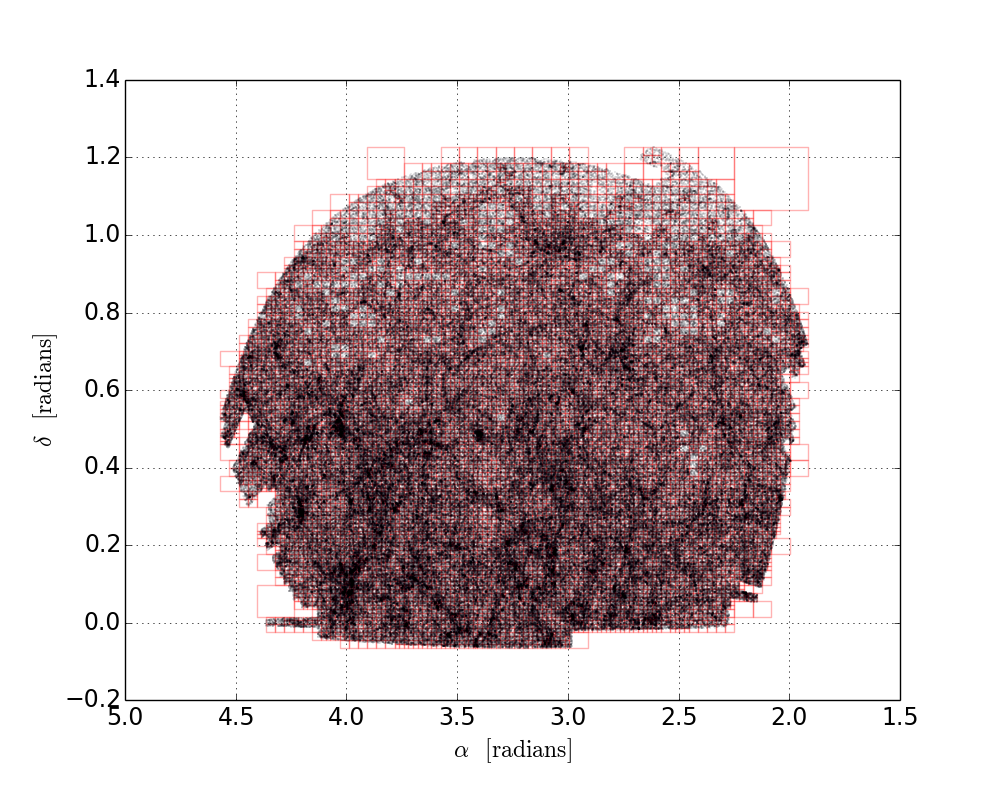
\includegraphics[width=0.7\linewidth]{figures/appendix/quadtree/quadtree.png}
    \caption{A simple illustration of a QuadTree generated for the SDSS
    adjoining block of galaxies. The tree is more refined in the regions at
higher surface density.\label{fig:quadtree}}
\end{figure}
%
\subsection{Searching in a given region}
%
To search in a given region, we go recursively through the tree structure, finding all
nodes that intersect it. An improvement can be done by computing if a node
is entirely contained by the searching region. If yes, we can directly use
the pointer to the identities array to include its points, without
descending more in the tree.

It is easy to determine whether the region and a node intersect is easy, since
they are defined as two rectangles in a two dimensional space.

The rectangular region is defined in the declination axis simply by taking
the central declination coordinate and adding it the angular distance for
the research region, since no distortions are present along this axis. For
the right ascension, we need to know the maximal separation between the
central point and the spherical circle generated by the angular distance.
For this extremal case point, it is clear that the corresponding meridian is
tangent to the spherical circle. So, in the spherical triangle formed by our
central point, the extremal point and the pole, we have a supplementary
constraint. The sinus formula applied to it gives us:
%
\begin{equation}
    \Delta\alpha = \mathrm{asin}\left(\cfrac{\sin d}{\cos\delta_0}\right)
\end{equation}
%
where $d$ is the angular radius inside which we are searching for points and
$\delta_0$ is the declination of the central point around which we search.
Our rectangular area is completely defined, and the intersections with the
nodes of the tree are easy to compute.

The case of the periodic search is complex. If the rectangular region fall
outside the periodic limits (inferior to 0 or superior to $2\pi$ in right
ascension on the celestial sphere), we need to duplicate the search region
and make the intersection with nodes for two regions instead of one. This is
a little time consuming but is the only way to handle correctly the periodic
case.
%
\subsection{$k$ nearest neighbors}
%
The $k$ nearest neighbors in the celestial sphere uses the implementation of
the search in a given region of the sky.

We find the leaf node to which our central point belongs to. A particular
attention must be done since we keep only non empty nodes. If the point
belongs to an empty one, we affect to it the parent node. In each case, we
take the parent node of the found node and search points inside it. Their
identities are added to a queue of size $k$ in ascending order of distance
to the central point.

We define a search region with this most distant point and fill again the
queue with points of this region. If the number of points found is inferior
to $k$, we take the parent node and redo the same computation until the
queue is entirely filled with the $k$ nearest neighbors.

\bartchapterimage{formulas}
\bartthumb{thumb_formulas}
\chapter{Formulas}

%\minitoc%

\section{Introduction}

In this appendix are described the formulas used in all computations realized during my thesis. Its just a simple way to share and
verify that the job id done correctly. References to those formulas are indicated too, in order to improve search when some doubts
are presents.\comments{Add a little more in the introduction.}

\section{Formulas}

\subsection{Cosmology}
Formulas which are related to the cosmology.

\noindent\rule{\linewidth}{1pt}
The luminosity distance is defined as the relation between the galaxy flux $S$ and its absolute luminosity
$L$ by:
\begin{equation}
	d_{\mathrm{lum}}=\sqrt{\cfrac{L}{4\pi{S}}}
\end{equation}
An analytical precise computations isn't possible, but numerical computations exist. Although precise, numerical recipes aren't
sufficiently fast in practice. Some other analytical approximations of this distance was created.

For example, in \citet{WU10}, an approximation good to 0.3\% is available for a range of values in $\Omega_\Lambda$ compatible
with WMAP and Planck results.In this approximation we have:
\begin{equation}
	d_{\mathrm{lum}}\pg{z}\pd=\cfrac{c}{3H_0}\cfrac{1+z}{\Omega_\Lambda^{1/6}\pg{1-\Omega_\Lambda}\pd^{1/3}}[\Psi\pg{x\pg{0,\Omega_\Lambda}\pd}\pd-\Psi\pg{x\pg{z,\Omega_\Lambda}\pd}\pd]
\end{equation}
with:
\begin{equation}
	\Psi\pg{x}\pd=3x^{1/3}{2^{2/3}}\left[1-\cfrac{x^2}{252}-\cfrac{x^4}{21060}\right]\\
\end{equation}
\begin{equation}
	x\pg{\alpha}\pd=\ln\pg{\alpha+\sqrt{\alpha^2+1}}\pd\\
\end{equation}
\begin{equation}
	\alpha\pg{z,\Omega_\Lambda}\pd=1+2\cfrac{\Omega_\Lambda}{1-\Omega_\Lambda}\cfrac{1}{\pg1+z\pd^3}
\end{equation}
The other distances are simply linked to this luminosity distance. The angular distance $d_{\mathrm{ang}}$ and the proper distance
$d_{\mathrm{pm}}$ are $d_{\mathrm{lum}}(z)={(1+z)}^2d_{\mathrm{ang}}(z)=(1+z)d_{\mathrm{pm}}(z)$.

\noindent\rule{\linewidth}{1pt}
The element of comoving volume is expressed using the Robertson-Walker metric as:
\begin{equation}
	\dd{V}=\cfrac{c}{H\pg{z}\pd}{d_{\mathrm{pm}}\pg{z}\pd}^2\dd{\Omega}\dd{z}
\end{equation}

\noindent\rule{\linewidth}{1pt}
The evolution of the fraction of matter, and dark energy is the following:
\begin{equation}
	\Omega_m\pg{z}\pd=\Omega_{m,0}\cfrac{\pg1+z\pd^3}{E\pg{z}\pd^2}
\end{equation}
\begin{equation}
	\Omega_\Lambda\pg{z}\pd=\cfrac{\Omega_{\Lambda,0}}{E\pg{z}\pd^2}
\end{equation}
where $z$ is the redshift and the subscript 0 refers to the actual value of the parameter.

\noindent\rule{\linewidth}{1pt}
The distance modulus represents the magnitude difference betweenthe observed flux of the galaxy and it would be if the galaxy was at
a distance of 10$pc$. So it's:
\begin{equation}
	DM\pg{z}\pd=5\log_{10}\pg\cfrac{d_{\mathrm{lum}}\pg{z}\pd}{10pc}\pd%
\end{equation}
where $z$ is the redshift of the galaxy and $d_{\mathrm{lum}}$ is the luminosity distance.

\noindent\rule{\linewidth}{1pt}
The apparent magnitude $m$ of galaxy in the perfect case where isn't K-correction, extinction\ldots, is just:
\begin{equation}\label{eq:magappdm}
	m=M+DM\pg{z}\pd%
\end{equation}
where $M$ is the absolute magnitude of this galaxy in the same band of $m$ and $DM(z)$ is the distance modulus at redshift $z$.

\noindent\rule{\linewidth}{1pt}
Magnitudes are defined at a given constant which is the same for each object so:
\begin{equation}
	M-M_\odot=-2.5\log_{10}\pg\cfrac{L}{L_\odot}\pd%
\end{equation}
where $M$ is absolute magnitude, $L$ the luminosity of the object and $\odot$ refers to Sun's quantities.
We can determined the luminosity by this relation which gives:
\begin{equation}
	\cfrac{L}{L_\odot}=10^{0.4\pg{M_\odot-M}\pd}
\end{equation}

\noindent\rule{\linewidth}{1pt}
For galaxies at a given redshift $z$, we can see all galaxies with an absolute magnitude
lower than (using equation (\ref{eq:magappdm})):
\begin{equation}
	m_{\mathrm{lim}}=M+DM\pg{z}\pd%
\end{equation}
where $m_{\mathrm{\lim}}$ is the apparent magnitude limit for a survey, and $M$ is the
absolute magnitude threshold to be seen at this redshift.

\noindent\rule{\linewidth}{1pt}
The virial radius $r_\Delta$ is defined as the radius at which the density is $\Delta$ times the critical density of the Universe.
So we have:
\begin{equation}\label{eq:radcrit}
	\rho\pg{r_\Delta}\pd=\Delta\rho_c
\end{equation}
with $\rho_c=\cfrac{3H\pg{z}\pd^2}{8\pi{G}}$.

If we suppose that the density is constant in this radius, we have:
\begin{equation}
	\Delta\cfrac{3H\pg{z}\pd^2}{8\pi{G}}=\cfrac{M_\Delta}{4\pi{r_\Delta}^3/3}
\end{equation}
where $M_\Delta$ is the virial mass.
We can now defined three quantities, the virial mass as:
\begin{equation}
	M_\Delta=\cfrac{\Delta{H\pg{z}\pd^2{r_\Delta}^3}}{2G}
\end{equation}
the virial radius as:
\begin{equation}
	r_\Delta=\pg\cfrac{2 G M_\Delta}{\Delta{H\pg{z}\pd^2}}\pd^{1/3}
\end{equation}
and the virial velocity as:
\begin{equation}
	v_\Delta=\sqrt{\cfrac{G M_\Delta}{r_\Delta}}=\sqrt{\cfrac{\Delta}{2}} H\pg{z}\pd{r_\Delta}
\end{equation}

\noindent\rule{\linewidth}{1pt}
Sometimes, the density at the virial radius isn't defined in relation with the critical density but instead with mean density of
the Universe. So the equation (\ref{eq:radcrit}) becomes:
\begin{equation}
	\rho\pg{r_\Delta}\pd=\Delta\rho_m=\Delta{\Omega_m}\rho_c
\end{equation}
We can treat this situation in the same way as previously, but formally with $\Delta\rightarrow\Delta\Omega_m$.

\noindent\rule{\linewidth}{1pt}
%\bibliographystyle{unsrtnat}
%\scriptsize{\cbleu{\bibliography{ref}}}

\cs{Halo mass functions}

A description of how to compute halo mass functions given simple models in some articles.

\fs{Theory}

\fss{Definition}

By definition, the halo mass function by unit of comobile volume is the number of halos with mass $M$ comprise between $M$ and
$M+\dd{M}$. If $N$ is the number of halos, the halo mass function $\phi\pg{M}\pd$ can be written:
\begin{eq}
	\phi\pg{M}\pd=\cfrac{\dd{N^2}}{\dd{M}\dd{V}}=\cfrac{\dd{n}}{\dd{M}}
\end{eq}
In this case, $n$ can be the comobile density of halos, or the CDF of the density. In the latter case, we have:
\begin{eq}
	n\pg{M,z}\pd=\int_0^M{\phi\pg{M,z}\pd\dd{M}}
\end{eq}
and so:
\begin{eq}
        \frac{\dd{n}}{\dd{M}}=\frac{\dd}{\dd{M}}\int_0^M{\phi\pg{M,z}\pd}\dd{M}=\frac{\dd}{\dd{M}}\pg{\Phi\pg{M,z}\pd}-{\Phi\pg{0,z}\pd}\pd={\phi\pg{M,z}\pd}
\end{eq}
where $\Phi$ is a primitive of $\phi$.

\fss{In practice}

Cosmological simulations give results with $f\pg\sigma\pd$ a fitted function on simulations. $\sigma\pg{M}\pd$ is the variance in
mass of the smoothed density fields. We can link this function to the halo mass function by:
\begin{eq}
	\phi\pg{M,z}\pd=\frac{\dd\ln{\sigma^{-1}}}{\dd{M}}\frac{\rho_m\pg{z}\pd}{M}{f\pg\sigma\pd}=\frac{\rho_m\pg{z}\pd}{M^2}\left|{{M}\frac{\dd\ln\sigma}{\dd{M}}}\right|{f\pg\sigma\pd}
\end{eq}
where the computation of $\sigma$ involves the power spectrum $P\pg{k}\pd$ and the filter for spectrum $\tilde{W}\pg{k}\pd$:
\begin{eq}
	\sigma^2\pg{M}\pd=\cfrac{1}{2\pi^2}\int_0^\infty{P\pg{k}\pd\tilde{W}\pg{k}\pd^2{k^2}\dd{k}}
\end{eq}
This form is time consuming for the computation of the halo mass function and model dependent. In \citet{2002MNRAS.331...98V}, there
is a good approximation for this formula which is resumed to:
\begin{eq}
        \sigma(M)=\sigma_8\frac{f(u)}{f(u_8)}
\end{eq}
with the function $f$:
\begin{eq}
        f(u)=\num{64,087}{(1+\num{1,074}{u^{\num{0,3}}}-\num{1,581}{u^{\num{0,4}}}+\num{0.954}{u^{\num{0.5}}}-\num{0.185}{u^{\num{0.6}}})}^{-10}
\end{eq}
and $u$, $u_8$ which are:
\begin{eqnarray}
        u&=&\num{3.804e-4}\Gamma\left(\frac{Mh}{\Omega_{m,0}}\right)^{1/3}\nonumber\\
        u_8&=&\num{32}\Gamma\nonumber\\
        \Gamma&=&\Omega_{m,0}h\exp\left[{-\Omega_b(1+\sqrt{2h}/\Omega_{m,0})}\right]\nonumber\\
\end{eqnarray}
Now, with this approximation, we can compute easily the derivative of $\sigma$ and:
\begin{eq}
        \pg{{M}\frac{\dd\ln\sigma}{\dd{M}}}\pd^{-1}+\undemi=\frac{\left(-0.000310111 X^{1.7}+0.00225895 X^{1.6}-0.00505879 X^{1.5}-0.1 X^{1.2}\right)}{\left(-0.000328357 X^{1.8}+0.00310111 X^{1.7}-0.0090358 X^{1.6}+0.0101176 X^{1.5}\right)}
\end{eq}
with:
\comments{Check if we can used directly the power spectrum in the calculation without
too many CPU time consuming...}
\begin{eq}
        X=\left(h \Omega _{m,0} e^{-\Omega _b \left(\frac{\sqrt{2} \sqrt{h}}{\Omega _{m,0}}+1\right)} \sqrt[3]{\frac{h M}{\Omega _{m,0}}}\right)
\end{eq}

\bartchapterimage{binary}
\bartthumb{thumb_binary}
\cs{Special functions}

\fs{Legendre elliptic integral function}

\fss{Introduction}

The Legendre elliptic integral function appears naturally when evaluationg distances like the luminosity distance in a flat
Universe. But the most of the time, this function isn't used directly because of the difficulty of implementation, and when it's
already adapted, this is not for all kinds of value. In following sections, we described how to use the NSWC implementation of
elliptic integrals.

\fss{Algorithm}


\fs{Incomplete gamma function}

\fss{Introduction}

By default, many algorithm used to compute incomplete gamma function doesn't allowed to have negative parameters
. By definition, the incomplete gamma function $\Gamma\pg{a,x}\pd$ is:
\begin{eq}
	\Gamma\pg{a,x}\pd=\int_x^\infty{e^{-t}{t^{a-1}}\dd{t}}
\end{eq}
when $a\leq0$, we can't compute this function with usual algorithms.
Moreover, we need to used an algorithm which doesn't use the "simple" gamma function $\Gamma\pg{a}\pd$:
\begin{eq}
	\Gamma\pg{a}\pd=\int_0^\infty{e^{-t}{t^{a-1}}\dd{t}}
\end{eq}
Indeed this function have singularities for negative values of $a$ where $a$ is an integer, as we can
see in figure (\ref{fig:gamma}).
\begin{figure}[hbtp]
	\centering
	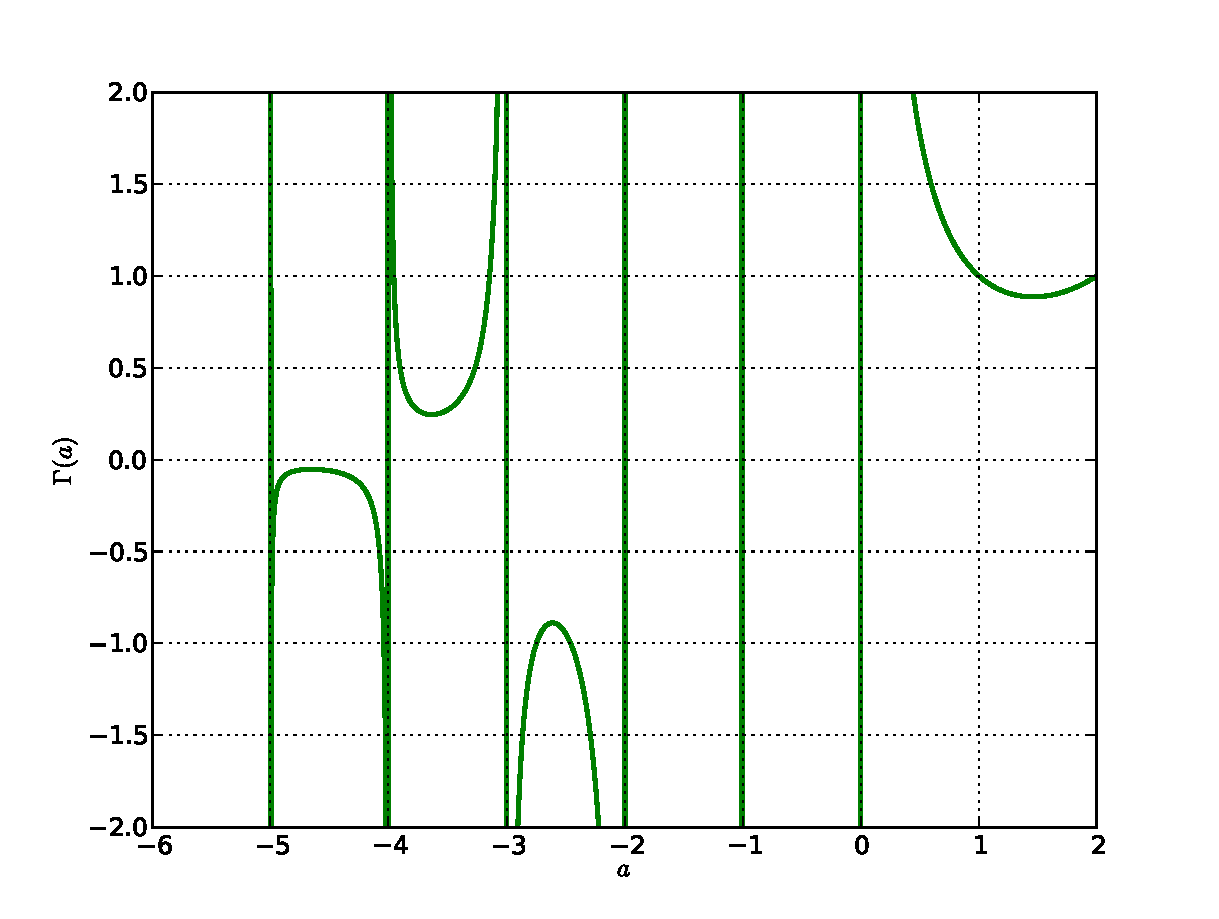
\includegraphics[width=0.5\linewidth]{gamma.pdf}
	\caption{\footnotesize{}The gamma function.}
	\label{fig:gamma}
\end{figure}
So we need an algorithm which not involves to use the gamma function for negative values. Here is described such algorithm.

\fss{Algorithm}

\fsss{Theory}

The best way to compute the incomplete gamma function for $a$ negative values is to use recurrence relations.
Let us define:
\begin{eq}
	\Gamma\pg{a+1,x}\pd=\int_x^\infty{e^{-t}{t^{a}}\dd{t}}
\end{eq}
Defining $u'=e^{-t}$ and $v=t^a$, we can use integration by parts:
\begin{eq}
	\Gamma\pg{a+1,x}\pd=\left[-e^{-t}{t^a}\right]_x^\infty + a \int_x^\infty{e^{-t}{t^{a-1}}\dd{t}}
\end{eq}
The all integrated part is always zero for all values of $a$ at infinity, and the second member of the right hand side
of the previous equation lets appear the definition of the incomplete gamma function.
So the recurrence relation for the incomplete gamma function is:
\begin{eq}
	\Gamma\pg{a+1,x}\pd=e^{-x}{x^a} + a \Gamma\pg{a,x}\pd
\end{eq}
We can see that computing the incomplete gamma function for $a<=0$ can be done with a recursive function
using the function at higher values of $a$.
\begin{eq}
	\Gamma\pg{a,x}\pd= \cfrac{ \Gamma\pg{a+1,x}\pd - e^{-x}{x^a} }{a}
\end{eq}
The previous equation shows that there is still a problem for integer values of $a$ because if $a=-2$
for example, at a moment in the recursion, we have a value of 0 for $a$ which create problems.
If we refer to \citet{abramowitz+stegun}, the definition of the elliptical integral is:
\begin{eq}
	E_n\pg{z}\pd=\int_1^\infty{e^{-zt}}{t^{-n}}\dd{t}
\end{eq}
for integer values of $n$. If we change the variable in the integral to $t'=zt$, we can rewrite the equation
to have:
\begin{eq}
	E_n\pg{z}\pd={z^{n-1}}\Gamma\pg{1-n,z}\pd
\end{eq}
so:
\begin{eq}
	\Gamma\pg{a,x}\pd={x^a}E_{1-a}\pg{x}\pd
\end{eq}
for $a\leq0$ and $a$ integer.
Now we have a good computation for the incomplete gamma function. But numerically, there is still a problem
near integer negative values of $a$. If $a$ is very close to an integer value, at a moment in the recursion,
$a$ is very small. So $1/a$ can be bigger than the overflow value for the machine. To avoid this, we add a
condition for $a$ when it is near zero.

An other definition of the incomplete gamma function is:
\begin{eq}
	\Gamma\pg{a,x}\pd=\Gamma\pg{a}\pd-\gamma\pg{a,x}\pd=\Gamma\pg{a}\pd\pg{1-P\pg{a,x}\pd}\pd
\end{eq}
with:
\begin{eq}
	\gamma\pg{a,x}\pd=\int_0^x{e^{-t}{t^{a}}\dd{t}}
\end{eq}
In \citet{NumericalRecipes} exists a precise computation of the function $P\pg{a,x}\pd$. We can remark that
this function isn't needed in the recursion if we have already access to a function which compute the
incomplete gamma function for positive values of $a$.

Following is described the algorithm for computing incomplete gamma function without loss of precision
and without numericals problems for negative values of $a$.

\fsss{Numerical}

%\begin{listing}[H]
\begin{minted}[bgcolor=griscode, linenos]{python}
def gammainc( a, x ):

	""" To compute the incomplete gamma function
	without loss of precision or without numerical
	problems. OF is the value of the overflow for
	the machine and expint( n, x ) the function
	which computes the integral function for n and x """

	import numpy as np

	if x >= 0. :

		if a <= 1. :

			if a == int( a ) or OF * abs( a ) < 1 :

				return x * int( a ) * \
					expint( 1 - int( a ), x )

			else :

				return ( gammainc( a + 1, x ) - \
					np.exp( -x ) * ( x ** a ) ) / a

		else :

			return gamma( a ) ( 1 - P( a, x ) )
			# or call the function which computes
			# the incomplete gamma function for
			# positive values of a
\end{minted}
%\end{listing}



\appendix

% adding files for the appendix
\bartchapterimage{heic0911c.jpg}
\chapter{Density profiles}
\label{cha:profiles}
\bartthumb{heic0911c.png}

\section{Introduction}

In this chapter, we provide details on the computation of the density profiles
and their derived quantities. We define here the different normalizations used
along the thesis for some popular density profiles.

\subsection{Definitions}

The number of galaxies in a sphere of radius $r$ with a density profile in
number $\nu(r)$ is the case of a spherical symmetry:
%
\begin{equation}
    N\left(r\right)=\int_0^r4\pi {r'}^2 \nu(r')\dd{r'}
\end{equation}

To start, we define some dimensionless functions to facilitate the
computations.
%
\begin{eqnarray}
    N\left(r\right)&=N\left(a\right){\widetilde{N}\left(r/a\right)}\nonumber\\
    \nu\left(r\right)&=
        \cfrac{N\left(a\right)}{4\pi{a^3}}
        \,\widetilde\nu\left(r/a\right)
\end{eqnarray}
%
with $a$ the radius at which the logarithmic slope of the density profile is
equal to $-2$. We also define the same relations for a
virial normalization.
%
\begin{eqnarray}
    N\left(r\right)&={N_v}\,{\widehat{N}\left(r/\rvir\right)}\nonumber\\
    \nu\left(r\right)&=
        \cfrac{N_v}{4\pi\rvir^3}\,\widehat\nu\left(r/\rvir\right)
\end{eqnarray}

We also define the concentration $c$ as the ratio between the virial radius
$\rvir$ and the radius $a$, i.e.\ $c=\rvir/a$. We define $\rvir=r_{200}$ for
simplicity.

\section{Density profiles}
\label{sec:density_profiles}

\subsection{\citet{NFW+97}}

The NFW density profile is:
%
\begin{equation}
    \nu \left(r\right) = \cfrac{\nu_0}{r {\left(r+a\right)}^2}
\end{equation}
%
with $\nu_0$ a constant density.

We can write by integrating previous relations with $\int_0^1
x^2\widetilde\nu\dd x=\int_0^1 x^2\widehat\nu\dd x$  and searching for the
constant $\nu_0$:
%
\begin{equation}
    \widetilde\nu\left(x\right)=\cfrac{1}{\ln2-1/2}
        \quad\cfrac{1}{x{\left(1+x\right)}^2}
\end{equation}
%
\begin{equation}
    \widetilde{N}\left(x\right)=\cfrac{1}{\ln2-1/2}
        \quad\left(\ln\left(1+x\right)-\cfrac{x}{x+1}\right)
\end{equation}
%
\begin{equation}
    \widehat\nu\left(x\right)=
        \cfrac{1}{\ln\left(1+c\right)-c/ \left(1+c\right)}
        \quad\cfrac{1}{x{\left(1/c+x\right)}^2}
\end{equation}
%
\begin{equation}
    \widehat{N}\left(x\right)=
        \cfrac{1}{\ln \left(1+c\right)-c/ \left(1+c\right)}
        \quad\left(\ln\left(1+xc\right)-\cfrac{xc}{xc+1}\right)
\end{equation}

\subsection{Einasto}
\label{sub:einasto}

For an Einasto density profile:
\begin{equation}
    \nu \left(r\right) = \nu_0 \exp
    \left[- {\left(\cfrac{r}{b}\right)}^{1/m}\right]
\end{equation}

Writing the definition of the $a$ radius with this density profile, we have:
%
\begin{equation}
    {\left(\cfrac{1}{b}\right)}^{1/m} = 2m{\left(\cfrac{1}{a}\right)}^{1/m}
\end{equation}
%
leading to the following normalizations:
%
\begin{equation}
    \widetilde\nu \left(x\right) = \cfrac{{\left(2m\right)}^{3m}}{m\gamma
    \left(3m, 2m\right)} \exp \left(-2mx^{1/m}\right)
\end{equation}
%
\begin{equation}
    \widetilde{N} \left(x\right) = \cfrac{\gamma \left(3m, 2m
    x^{1/m}\right)}{\gamma \left(3m, 2m\right)}
\end{equation}
%
\begin{equation}
    \widehat\nu \left(x\right) = \cfrac{{\left(2m\right)}^{3m}}{m\gamma
    \left(3m, 2m c^{1/m}\right)} \exp \left(-2m{\left(xc\right)}^{1/m}\right)
\end{equation}
%
\begin{equation}
    \widehat{N} \left(x\right) = \cfrac{\gamma \left(3m, 2m
        {\left(xc\right)}^{1/m}\right)}{\gamma \left(3m, 2m c^{1/m}\right)}
\end{equation}

\subsection{Generalized NFW}
\label{sub:generalized_nfw}

If any previous density profiles isn't sufficient to describe the distribution
of dark matter particles or galaxies inside the halos, a solution is possibly
to fit a generalized NFW profile, whose the density is:
%
\begin{equation}
    \nu \left(r\right) =
    \cfrac{\nu_0}{r^\alpha{\left(r+a\right)}^{\beta-\alpha}}
\end{equation}

In this case:
%
\begin{equation}
    \widetilde{N} \left(x\right) = \cfrac{%
        \mathcal{B}_{-x} \left(3-\alpha, 1+\alpha-\beta\right)}
    {\mathcal{B}_{-1} \left(3-\alpha, 1+\alpha-\beta\right)}
\end{equation}
%
therefore:
%
\begin{equation}
    \widetilde\nu \left(x\right) = \cfrac{1}
    {{\left(-1\right)}^{\alpha+1}
        \mathcal{B}_{-1} \left(3-\alpha, 1+\alpha-\beta\right)}
    \quad\cfrac{1}
    {x^\alpha {\left(1+x\right)}^{\beta-\alpha}}
\end{equation}
%
For the virial normalization:
%
\begin{equation}
    \widehat{N} \left(x\right) = \cfrac{%
        \mathcal{B}_{-xc} \left(3-\alpha, 1+\alpha-\beta\right)}
    {\mathcal{B}_{-c} \left(3-\alpha, 1+\alpha-\beta\right)}
\end{equation}
%
\begin{equation}
    \widehat\nu \left(x\right) = \cfrac{1}
    {{\left(-1\right)}^{\alpha+1}
        \mathcal{B}_{-c} \left(3-\alpha, 1+\alpha-\beta\right)}
    \quad\cfrac{1}
    {{\left(xc\right)}^\alpha {\left(1+xc\right)}^{\beta-\alpha}}
\end{equation}
%
where $\mathcal{B}$ is the function defined as:
%
\begin{equation}
    \mathcal{B} \left(a, b\right) =
    \cfrac{\Gamma \left(a\right) \Gamma \left(b\right)}
    {\Gamma \left(a+b\right)} =
    \int_0^1 t^{a-1} {\left(1+t\right)}^{b-1} \dd t
\end{equation}
%
and its incomplete version is:
%
\begin{equation}
    \mathcal{B}_z \left(a, b\right) =
    \int_0^z t^{a-1} {\left(1+t\right)}^{b-1} \dd t
\end{equation}

\section{Radial velocity dispersion}
\label{sec:radial_velocity_dispersion}

Galaxies in groups (and their associated dark matter halos) are assumed to be a
system of particles only submitted to the gravitation. Neglecting mergers and
other physical processes inside galaxy groups, the number of galaxies doesn't
evolve in phase space, and the distribution function is constant along the
evolution of the system. In this case, we can use the collisionless Boltzmann
equation to extract dynamical properties of galaxy groups.

The Jeans equation is the first velocity momentum of the Boltzmann equation. In a
spherical symmetry, assuming stationarity, the Jeans equation is:
%
\begin{equation}
    \label{eq:jeans}
    \ddp{\left[\nu(r)\sigma_r^2(r)\right]}{r} +
    \cfrac{2\mybeta}{r}\left[\nu(r)\sigma_r^2(r)\right]=
    -\nu(r)\cfrac{GM(r)}{r^2}
\end{equation}
%
where $\beta \left(r\right)$ is the radial profile of velocity anisotropy
$\beta = 1 - \sigma_\theta^2/\sigma_r^2$.

We can compute the radial velocity dispersion using \bartrefequation{jeans} for
a spherical system at equilibrium. The solution to this equation is given by:
%
\begin{equation}
    \myprofil\sigma_r^2(r)=
    \int_r^\infty K_r(r,s)\nu(s)\cfrac{GM(s)}{s^2}\,\dd{s}
\end{equation}
%
with $K_r(r,s)$ the kernel of the integral defined as:
%
\begin{equation}
    K_r(r,s)=\exp\left[2\int_r^s\mybeta\cfrac{\dd{t}}{t}\right]
\end{equation}

There are two ways of normalizing the radial velocity dispersion according to
the normalization used for the density and mass profiles. We show it for the
virial normalization for illustration:
%
\begin{equation}
    \label{eq:sigma_norm}
    \widehat\sigma_r^2(x)= \cfrac{1}{\widehat\nu \left(x\right)}
    \int_x^\infty K_r(x,s)\widehat\nu(s)\cfrac{\widehat{M}(s)}{s^2}\,\dd s
\end{equation}
%
with:
%
\begin{equation}
    \sigma_r^2(r) = \cfrac{GM_v}{\rvir}\,\widehat\sigma_r^2(r/\rvir)
\end{equation}

We are interested only in the NFW profile in the thesis, since it is accurate
enough to adjust the model. If we want an analytical form for $\sigma_r
\left(r\right)$, we need to choose a model for the anisotropy profile $\beta
\left(r\right)$. We provide here some expressions of the radial velocity
dispersion, assuming the NFW density profile, for a useful anisotropy model.

\subsection{\citet{ML+05}}
\label{sub:ml05}

This model is of the form:
%
\begin{equation}
    \beta \left(r\right) = \undemi\cfrac{r}{r+b}
\end{equation}
%
where $b$ is a characteristic radius of the model. Introducing this expression
in \bartrefequation{sigma_norm}, we obtain:
%
\begin{align}
    \widetilde\sigma_r^2(x)=&
        -\frac{1}{3 x (1+r x)
        {(-1+\ln\left(4\right))}^2}2
        \left(-\frac{1}{2}+\ln\left(2\right)\right)\nonumber\\
    &\left(x \left(3+x \left(\pi ^2 (-3+2 r)
        {(1+x)}^2-3 (-9+5 r-7 x+4 r x)
        \right)\right.\vphantom{\ln\left(1+\frac{1}{x}\right)}\right.
        \nonumber\\
    &\left.-3 x^3 \ln\left(1+\frac{1}{x}\right)+3 x (1+2 x)
        \ln\left(x\right)\right)\nonumber\\
    & -3 (1+2 x (-1-2 x (2+x)+r (1+x) (1+2 x)))
        \ln\left(1+x\right)+3 (-3+2 r) {\left(x+x^2\right)}^2
        \ln{\left(1+x\right)}^2\nonumber\\
    & \left.+6 (-3+2 r) x^2 {(1+x)}^2
        Li_2\left(-x\right)\vphantom{\ln\left(1+\frac{1}{x}\right)}\right)
        \nonumber\\
\end{align}
\begin{align}
    \widehat\sigma_r^2(x)=&
        \frac{1}{6 x (1+r x) \left(-1+\frac{1}{1+c}+\ln c\right)}
        \left(c x \left(-3+x \left(3 c \left(-9+\pi ^2\right)+
        \left(15-2 \pi ^2\right) r\right.\right.
        \vphantom{{(1+c x)}^2}\right.\\
    &\left. -4 c \left(-3+\pi ^2\right) r x+
        3 c^3 \pi ^2 x^2+c^2 x \left(-21+\pi ^2 (6-2 r x)\right)\right)\\
    & \left.+6 c^3 x^3 {\rm arccoth} \left(1+2 c x\right)-
        3 c x (1+2 c x) \ln\left(c x\right)\right)\\
    &+3(1+2 x (r+c (-1+x (-4 c+3 r+2 c (-c+r) x))))
        \ln\left(1+c x\right)\\
    &\left.+3c(3 c-2 r) x^2 {(1+c x)}^2 {\left(\ln\left(1+c x\right)\right)}^2+
    6 c (3 c-2 r) x^2 {(1+c x)}^2 \mathrm{Li_2}\left(-c x\right)\right)\\
\end{align}

\section{Line of sight velocity variance}

We will compute in this section the line of sight velocity dispersion of
galaxies in a general spherical density profile, and then compute it
specifically for an NFW profile. This is useful to make cuts at
$\pm\kappa\sigma_\mathrm{LOS} \left(R\right)$ in the \pps{}.

By definition, the variance is the mean of the squared quantity. We use a
general density profile which is invariant under rotations $\nu{(r)}$. In our
case, we make this mean on the line of sight, so:
%
\begin{equation}
    \sigma_\mathrm{LOS}^2\left({R}\right)=
    \cfrac{\int_{-\infty}^{\infty}{v_\mathrm{LOS}^2}\nu{(r)}\,\dd{z}}
    {\int_{-\infty}^{\infty}\nu{(r)}\,\dd{z}}
\end{equation}
%
But in the group, $r^2=R^2+z^2$ so:
%
\begin{equation}
    \sigma_\mathrm{LOS}^2\left({R}\right)=
    \cfrac{2\int_{R}^{r_{\max}}{v_\mathrm{LOS}^2}
    \cfrac{\nu{(r)}{r}}{\sqrt{r^2-R^2}}\,\dd{r}}
    {2\int_{R}^{r_{\max}}\cfrac{\nu{(r)}{r}}{\sqrt{r^2-R^2}}\,\dd{r}}
\end{equation}
%
The denominator is by definition the projected density surface along the line
of sight and we denote it
%
\begin{equation}
    \Sigma(R) = 2\int_{R}^{r_{\max}}\cfrac{\nu{(r)}{r}}{\sqrt{r^2-R^2}}\,\dd{r}
\end{equation}
%
Normally the integration is for $r_{\max}\rightarrow\infty$ but in our case we
want to restrict to a limited region in the group (to the virial sphere
precisely).

In the same coordinate system as previously, the line of sight velocity can be
expressed in spherical coordinates as:
%
\begin{equation}
    v_{\mathrm{LOS}} = v_r \cos\theta - v_\theta \sin\theta
\end{equation}
%
We suppose that we are at the equilibrium and so that there is no flow in the
group in consequence we can neglect means of velocities. In terms of velocity
variance we have now:
%
\begin{equation}
    \mysigma\mysiglos = 2\int_R^{r_{\max}}
    \left({\sigma_r^2(r)\cos^2\theta+\sigma_\theta^2\sin^2\theta}\right)
    \cfrac{\nu{(r)}{r}}{\sqrt{r^2-R^2}}\,\dd{r}
\end{equation}
%
If we want to use the anisotropy parameter
$\mybeta=1-\sigma_\theta^2(r)/\sigma_r^2(r)$ in case of sphericity, we can
write:
%
\begin{equation}
    \mysigma\mysiglos = 2\int_R^{r_{\max}}
    \left({1-\mybeta\cfrac{R^2}{r^2}}\right)
    \cfrac{\nu{(r)}{\sigma_r^2(r)}{r}}{\sqrt{r^2-R^2}}\,\dd{r}
\end{equation}

We can compute the radial velocity dispersion using the Jeans equation for a
spherical system at equilibrium.

\subsection{\citet{ML+05} anisotropy}

With the decomposition of the integral over the domain of integration, we can
write:
%
\begin{align}
    \Sigma{(R)}{\sigma_\mathrm{LOS}}^2{(R)}=&
        2\int_R^{r_v}{\cfrac{\left({s+a}\right)}{s^2}{\nu(s)}{G}{M(s)}}{\dd{s}}
        \nonumber\\
    &\times
        \left(\int_R^s{\left(\cfrac{r}{r+a}-\undemi
        {\left(\cfrac{R}{r+a}\right)}^2\right)
        \cfrac{1}{\sqrt{r^2-R^2}}\dd{r}}\right)\nonumber\\
    &+2\int_{r_v}^{\infty}
        \cfrac{\left({s+a}\right)}{s^2}\nu(s){G}{M(s)}\dd{s}\nonumber\\
    &\times
        \left(\int_R^{r_v}
            \left(\cfrac{r}{r+a}-\undemi{\left(\cfrac{R}{r+a}\right)}^2\right)
            \cfrac{1}{\sqrt{r^2-R^2}}\dd{r}\right)
\end{align}
%
where we are setting $r_{\max}$ to $r_v$. So now we can write:
%
\begin{align}
    {\sigma_\mathrm{LOS}}^2{(R)}=&{v_v}^2\cfrac{c/2}{\widetilde{M}{(c)}\widetilde{\Sigma}{(R/a,c)}}\nonumber\\
    &\times\left(\int_{R/a}^c{{K}\left({x\cfrac{a}{R},\cfrac{a}{R}}\right)}\widetilde{\nu}{(x)}
    \cfrac{\widetilde{M}{(x)}}{x}\dd{x}+I\left({c\cfrac{a}{R},\cfrac{a}{R}}\right){J(c)}\right)
\end{align}
%
\begin{equation}
    I(u,u_a)=\left\{\begin{array}{lr}
        -u_a{\rm{sign}}(u_a-1)\cfrac{{u_a}^2-1/2}{|{u_a}^2-1|^{3/2}}{C^{-1}\left(\cfrac{1+u{u_a}}{u+u_a}\right)}&\\
        \hspace{5em}+{\rm{acosh}}{u}+\cfrac{1/2}{u_a+u}\cfrac{\sqrt{u^2-1}}{{u_a}^2-1},&{u_a}\neq1\\
        {\rm{acosh}}{u}-\sqrt{\cfrac{u-1}{u+1}}\left(\cfrac{8+7u}{6(1+u)}\right),&{u_a}=1\\
    \end{array}\right.
\end{equation}
%
with:
%
\begin{equation}
    K(u,u_a)=\left({1+\frac{u_a}{u}}\right){I(u,u_a)}
\end{equation}
%
and:
%
\begin{equation}
    C^{-1}(X)=\left\{\begin{array}{lr}
        {\rm{acosh}}{X}&u_a>1\\
        {\rm{acos}}{X}&u_a<1\\
    \end{array}\right.
\end{equation}
%
We also have an other integral:
%
\begin{equation}
    J(y)=\int_y^{\infty}\frac{x+1}{x^2}\widetilde{\nu}{(x)}\widetilde{M}{(x)}\dd{x}
\end{equation}
%
In the case of an NFW profile, this can be expressed in an analytical way:
%
\begin{align*}
    J(y)=&
        \frac{2}{3{y^2}(1+y){\left(\ln{4}-1\right)}^2}
        \left(y\left(-3+y\left(-9+\pi^2\left(1+y\right)\right)\right)\right.\\
    &+3{y^3}\ln\left(1+\frac{1}{y}\right)+3\ln\left(1+y\right)
            \left(1-y+y^2\left(1+y\right)\ln\left(1+y\right)\right)\\
    &\left.-3{y^2}\ln\left({y}\left(1+y\right)\right)+6{y^2}
        \left(1+y\right){\dilog{-y}}\right)\\
\end{align*}
%
where the dilogarithm function is defined in our case as:
%
\begin{equation}
    \dilog{z}=-\int_0^1\cfrac{\ln{(1-zt)}}{z}\,\dd{t}
\end{equation}

For the NFW model, \citet{MBM+10} provide the expression of
$\widetilde{\Sigma}$:
%
\begin{multline}
    \widetilde{\Sigma}(X,c)=\cfrac{1}{2\ln2-1}\int_X^c\cfrac{\dd{x}}{{(1+x)}^2\sqrt{x^2-X^2}}\\
    =\cfrac{1}{2\ln2-1}\begin{cases}
        \cfrac{1}{{(1-X^2)}^{3/2}}
        \cosh^{-1}\left[\cfrac{c+X^2}{(c+1)X}\right]-
        \cfrac{1}{(c+1)}\cfrac{\sqrt{c^2-X^2}}{1-X^2} &\text{if } 0<X<1 \\
    \cfrac{\sqrt{c^2-1}(c+2)}{3{(c+1)}^2} &\text{if } X=1<c\\
    \cfrac{1}{(c+1)}\cfrac{\sqrt{c^2-X^2}}{X^2-1}-
    \cfrac{1}{{(X^2-1)}^{3/2}}
    \cos^{-1}\left[\cfrac{c+X^2}{(c+1)X}\right] &\text{if } 1<X<c\\
    0 &\text{if } X=0\,\text{or}\,X>c
    \end{cases}
\end{multline}

% vim: set tw=79 : set concealcursor=

%
\chapter{Line of sight velocity variance}

\newcommand{\mybeta}{%
\beta(r)%
}
\newcommand{\mysigma}{%
\Sigma(r)%
}
\newcommand{\mysiglos}{%
\sigma_{\mathrm{LOS}}^2(R)%
}
\newcommand{\myprofil}{%
\nu(r)%
}

\section{Introduction}

We will compute in this section the line of sight velocity dispersion
of galaxies in a general spherical density profile, and then compute it
specifically for an NFW profile.

This useful to make cuts at some sigma in the velocity profile to check
where is the most important part of a group.

\section{Calculus}

By definition, the variance is the mean of the squared quantity under the
assumption of a distribution function.
We use a general density profile which is invariant under rotations $\nu{(r)}$.
In our case, we make this mean on the line of sight, so:
\[
\sigma_{LOS}^2\pg{R}\pd=\cfrac{\int_{-\infty}^{\infty}{v_{LOS}^2}\nu{(r)}\dd{z}}
{\int_{-\infty}^{\infty}\nu{(r)}\dd{z}}
\]
But in the group $r^2=R^2+z^2$ so:
\[
\sigma_{LOS}^2\pg{R}\pd=\cfrac{2\int_{R}^{r_{\mathrm{max}}}{v_{LOS}^2}\cfrac{\nu{(r)}{r}}{\sqrt{r^2-R^2}}\dd{r}}
{2\int_{R}^{r_{\mathrm{max}}}\cfrac{\nu{(r)}{r}}{\sqrt{r^2-R^2}}\dd{r}}
\]
The denominator is by definition the projected density surface along the line of sight
and we denote it
\[
\Sigma(R) = 2\int_{R}^{r_{\mathrm{max}}}\cfrac{\nu{(r)}{r}}{\sqrt{r^2-R^2}}\dd{r}
\]
Normally the integration is for $r_{\mathrm{max}}\rightarrow\infty$ but in our case
we want to restrict to a limited region in the group (to virial sphere precisely).

In the same coordinate system as previously, the line of sight velocity can be expressed
in spherical coordinates as:
\[
v_{\mathrm{LOS}} = v_r \cos\theta - v_\theta \sin\theta
\]
We suppose that we are at the equilibrium and so that there is
no flow in the group in consequence we can neglect means of velocities.
In terms of velocity variance we have now:
\[
\mysigma\mysiglos = 2\int_R^{r_{\mathrm{max}}}
\pg{\sigma_r^2(r)\cos^2\theta+\sigma_\theta^2\sin^2\theta}\pd
\cfrac{\nu{(r)}{r}}{\sqrt{r^2-R^2}}\dd{r}
\]
If we want to use the anisotropy parameter $\mybeta=1-\sigma_\theta^2(r)/\sigma_r^2(r)$
in case of sphericity\postit{Check word sphericity!}{5}, we can write:
\[
\mysigma\mysiglos = 2\int_R^{r_{\mathrm{max}}}
\pg{1-\mybeta\cfrac{R^2}{r^2}}\pd
\cfrac{\nu{(r)}{\sigma_r^2(r)}{r}}{\sqrt{r^2-R^2}}\dd{r}
\]

We can compute the radial velocity dispersion using the Jeans equation
for a spherical system at equilibrium.
\[
\ddp{\pg\nu(r)\sigma_r^2(r)\pd}{r} + \cfrac{2\mybeta}{r}\pg\nu(r)\sigma_r^2(r)\pd=
-\nu(r)\cfrac{GM(r)}{r^2}
\]
The solution to this equation is given by:
\[
\myprofil\sigma_r^2(r)=\int_r^{r_{\mathrm{max}}}K_r(r,s)\nu(s)\cfrac{GM(s)}{s^2}\dd{s}
\]
with $K_r(r,s)$ the kernel of the integral defined as:
\[
K_r(r,s)=\exp\left[2\int_r^s\mybeta\cfrac{\dd{t}}{t}\right]
\]
\begin{figure}[H]
    \centering
    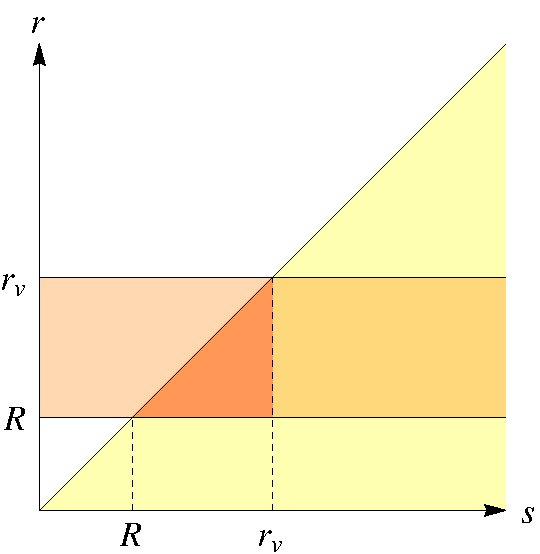
\includegraphics[width=0.5\linewidth]{domint}
    \caption{\footnotesize{}Integration domain for the line of sight radial dispersion.}
    \label{fig:domint}
\end{figure}

\subsection{Supposing \citet{ML05} anisotropy}
With the decomposition of the integral over the domain of integration, we can write
\begin{eqnarray}
    &&\Sigma{(R)}{\sigma_{LOS}}^2{(R)}=2\int_R^{r_v}{\frac{\pg{s+a}\pd}{s^2}{\nu(s)}{G}{M(s)}}{\dd{s}}\nonumber\\
    &\times&\pg\int_R^s{\pg\frac{r}{r+a}-\undemi\pg\frac{R}{r+a}\pd^2\pd\frac{1}{\sqrt{r^2-R^2}}\dd{r}}\pd\nonumber\\
    &+&2\int_{r_v}^{\infty}{\frac{\pg{s+a}\pd}{s^2}{\nu(s)}{G}{M(s)}}{\dd{s}}\nonumber\\
    &\times&\pg\int_R^{r_v}{\pg\frac{r}{r+a}-\undemi\pg\frac{R}{r+a}\pd^2\pd\frac{1}{\sqrt{r^2-R^2}}\dd{r}}\pd\nonumber\\
\end{eqnarray}
where we are setting $r_{\mathrm{max}}$ to $r_v$.
So now we can write using the fact that $4a\nu(a)\widetilde{\Sigma}(R/a,c)$:
\begin{eqnarray}
    &&{\sigma_{LOS}}^2{(R)}={v_v}^2\frac{c/2}{\widetilde{M}{(c)}\widetilde{\Sigma}{(R/a,c)}}\nonumber\\
    &\times&\pg\int_{R/a}^c{{K}\pg{x\frac{a}{R},\frac{a}{R}}\pd}\widetilde{\nu}{(x)}
    \frac{\widetilde{M}{(x)}}{x}\dd{x}+I\pg{c\frac{a}{R},\frac{a}{R}}\pd{J(c)}\pd\nonumber\\
\end{eqnarray}
\begin{equation}
    I(u,u_a)=\left\{\begin{array}{lr}
        -u_a{\rm{sign}}(u_a-1)\frac{{u_a}^2-1/2}{|{u_a}^2-1|^{3/2}}{C^{-1}\pg\frac{1+u{u_a}}{u+u_a}\pd}&\\
        \hspace{5em}+{\rm{acosh}}{u}+\frac{1/2}{u_a+u}\frac{\sqrt{u^2-1}}{{u_a}^2-1},&{u_a}\neq1\\
        {\rm{acosh}}{u}-\sqrt{\frac{u-1}{u+1}}\pg\frac{8+7u}{6(1+u)}\pd,&{u_a}=1\\
    \end{array}\right.
\end{equation}
with:
\begin{eq}
        K(u,u_a)=\pg{1+\frac{u_a}{u}}\pd{I(u,u_a)}
\end{eq}
and:
\begin{eq}
    C^{-1}(X)=\left\{\begin{array}{lr}
        {\rm{acosh}}{X}&u_a>1\\
        {\rm{acos}}{X}&u_a<1\\
    \end{array}\right.
\end{eq}
We have too an other integral:
\begin{eq}
        J(y)=\int_y^{\infty}\frac{x+1}{x^2}\widetilde{\nu}{(x)}\widetilde{M}{(x)}\dd{x}
\end{eq}
In the case of an NFW profile, this can be expressed in an analytical way:
\begin{align*}
        J(y)&=\frac{2}{3{y^2}(1+y)\pg\ln{4}-1\pd^2}\pg{y}\pg-3+y\pg-9+\pi^2\pg1+y\pd\pd\pd\right.\\
        &+3{y^3}\ln\pg1+\frac{1}{y}\pd+3\ln\pg1+y\pd\pg1-y+y^2\pg1+y\pd\ln\pg1+y\pd\pd\\
        &\left.-3{y^2}\ln\pg{y}\pg1+y\pd\pd+6{y^2}\pg1+y\pd{\dilog{-y}}\pd\\
\end{align*}
where the dilogarithm function is defined in our case as:
\[
\dilog{z}=-\int_0^1\cfrac{\ln{(1-zt)}}{z}\dd{t}
\]

Still in the case of the NFW profil, in \citet{MBM10} there is the expression of $\widetilde{\Sigma}$:
\begin{multline}
    \widetilde{\Sigma}(X,c)=\cfrac{1}{2\ln2-1}\int_X^c\cfrac{\dd{x}}{{(1+x)}^2\sqrt{x^2-X^2}}\\
    =\cfrac{1}{2\ln2-1}\begin{cases}
        \cfrac{1}{{(1-X^2)}^{3/2}}
        \cosh^{-1}\left[\cfrac{c+X^2}{(c+1)X}\right]-
        \cfrac{1}{(c+1)}\cfrac{\sqrt{c^2-X^2}}{1-X^2} &\text{if } 0<X<1 \\
    \cfrac{\sqrt{c^2-1}(c+2)}{3{(c+1)}^2} &\text{if } X=1<c\\
    \cfrac{1}{(c+1)}\cfrac{\sqrt{c^2-X^2}}{X^2-1}-
    \cfrac{1}{{(X^2-1)}^{3/2}}
    \cos^{-1}\left[\cfrac{c+X^2}{(c+1)X}\right] &\text{if } 1<X<c\\
    0 &\text{if } X=0\text{ or }X>c
    \end{cases}
\end{multline}

\bartchapterimage{trees.jpg}
\chapter{QuadTree on celestial sphere}
\label{cha:quadtree}
\bartthumb{trees.png}

\section{Introduction}

The extraction of galaxy groups from redshift space involves various algorithms
to search for galaxies in a given region of the sky. Methods as those used in
numerical simulations for searching dark matter halos can be applied. Such
techniques often use a partition of the space to make a brute force computation
of the distance between particles only on a small portion of the three
dimensional space. Same partitioning of the celestial sphere can be done, but
the non-euclidean metric of celestial coordinates make the task a little
harder.

\section{QuadTree}

The principle of the QuadTree is to make a partition of the space (celestial
sphere in our case). Each created partition will be partitioned too if the
number of galaxies in it is superior to a limit we define at the creation of
the QuadTree. If the number of levels in the refinement is superior to a given
limit, we stop the refinement.

This is clearly a tree structure, since the partitions, called nodes, are
subdivided into other nodes. This allow to rapidly search for galaxies in a
given region since we can easily determine which node intersect a given region.

\subsection{Construction}

The construction is straightforward with the description above. We start by
defining the limits in the $(\alpha, \delta)$ plane for the region to refine.
This region is the root node. Then, the following instructions are applied
recursively.

\begin{itemize}
    \item We determine in which child node each point is falling inside. We
        keep an array of the identities of points in the tree to which each
        node point to. In this array, identities are ordered according to the
        node of the point. So, at the end of the tree construction, the array
        of the identities will be structured in the same as the tree, allowing
        for optimization of the memory and for future searches of points.
    \item If the maximal level of refinement is reached, we no longer subdivide
        the node.
    \item If the number of points in the child node is superior to the fixed
        limit, we subdivide the node in four other nodes.
    \item Go to the brother of the node.
\end{itemize}
%
For optimization, we keep just nodes that are not empty, linking together
brother nodes.

During the construction of the node, we also keep the information of their
spatial geometry such as extremal coordinates in right ascension and
declination, center position, half width in each axis to avoid useless
computations when searching points on the celestial sphere.

At this stage, we make a simple partition of the space as in any other
QuadTree, without caring about the special metric involved.

An illustration of a QuadTree generated for the galaxies in the adjoining
block of the SDSS is shown in Figure~\ref{fig:quadtree}.
%
\begin{figure}
    \centering
    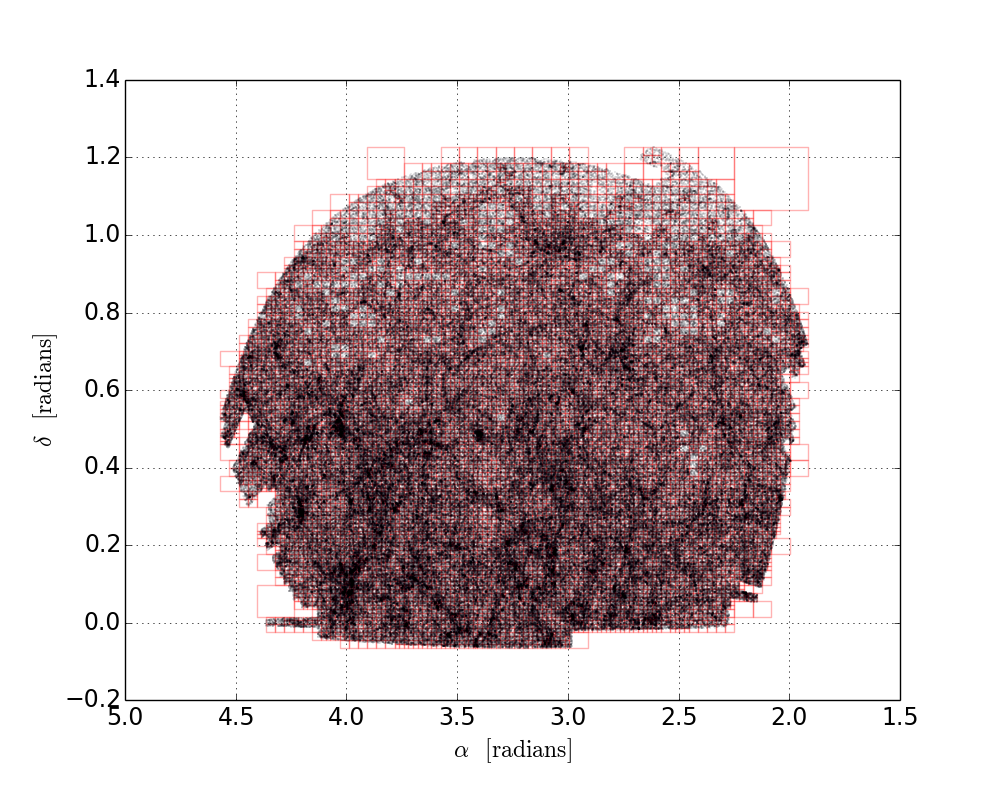
\includegraphics[width=0.7\linewidth]{figures/appendix/quadtree/quadtree.png}
    \caption{A simple illustration of a QuadTree generated for the SDSS
    adjoining block of galaxies. The tree is more refined in the regions at
higher surface density.\label{fig:quadtree}}
\end{figure}
%
\subsection{Searching in a given region}
%
To search in a given region, we go recursively through the tree structure, finding all
nodes that intersect it. An improvement can be done by computing if a node
is entirely contained by the searching region. If yes, we can directly use
the pointer to the identities array to include its points, without
descending more in the tree.

It is easy to determine whether the region and a node intersect is easy, since
they are defined as two rectangles in a two dimensional space.

The rectangular region is defined in the declination axis simply by taking
the central declination coordinate and adding it the angular distance for
the research region, since no distortions are present along this axis. For
the right ascension, we need to know the maximal separation between the
central point and the spherical circle generated by the angular distance.
For this extremal case point, it is clear that the corresponding meridian is
tangent to the spherical circle. So, in the spherical triangle formed by our
central point, the extremal point and the pole, we have a supplementary
constraint. The sinus formula applied to it gives us:
%
\begin{equation}
    \Delta\alpha = \mathrm{asin}\left(\cfrac{\sin d}{\cos\delta_0}\right)
\end{equation}
%
where $d$ is the angular radius inside which we are searching for points and
$\delta_0$ is the declination of the central point around which we search.
Our rectangular area is completely defined, and the intersections with the
nodes of the tree are easy to compute.

The case of the periodic search is complex. If the rectangular region fall
outside the periodic limits (inferior to 0 or superior to $2\pi$ in right
ascension on the celestial sphere), we need to duplicate the search region
and make the intersection with nodes for two regions instead of one. This is
a little time consuming but is the only way to handle correctly the periodic
case.
%
\subsection{$k$ nearest neighbors}
%
The $k$ nearest neighbors in the celestial sphere uses the implementation of
the search in a given region of the sky.

We find the leaf node to which our central point belongs to. A particular
attention must be done since we keep only non empty nodes. If the point
belongs to an empty one, we affect to it the parent node. In each case, we
take the parent node of the found node and search points inside it. Their
identities are added to a queue of size $k$ in ascending order of distance
to the central point.

We define a search region with this most distant point and fill again the
queue with points of this region. If the number of points found is inferior
to $k$, we take the parent node and redo the same computation until the
queue is entirely filled with the $k$ nearest neighbors.

\bartchapterimage{formulas}
\bartthumb{thumb_formulas}
\chapter{Formulas}

%\minitoc%

\section{Introduction}

In this appendix are described the formulas used in all computations realized during my thesis. Its just a simple way to share and
verify that the job id done correctly. References to those formulas are indicated too, in order to improve search when some doubts
are presents.\comments{Add a little more in the introduction.}

\section{Formulas}

\subsection{Cosmology}
Formulas which are related to the cosmology.

\noindent\rule{\linewidth}{1pt}
The luminosity distance is defined as the relation between the galaxy flux $S$ and its absolute luminosity
$L$ by:
\begin{equation}
	d_{\mathrm{lum}}=\sqrt{\cfrac{L}{4\pi{S}}}
\end{equation}
An analytical precise computations isn't possible, but numerical computations exist. Although precise, numerical recipes aren't
sufficiently fast in practice. Some other analytical approximations of this distance was created.

For example, in \citet{WU10}, an approximation good to 0.3\% is available for a range of values in $\Omega_\Lambda$ compatible
with WMAP and Planck results.In this approximation we have:
\begin{equation}
	d_{\mathrm{lum}}\pg{z}\pd=\cfrac{c}{3H_0}\cfrac{1+z}{\Omega_\Lambda^{1/6}\pg{1-\Omega_\Lambda}\pd^{1/3}}[\Psi\pg{x\pg{0,\Omega_\Lambda}\pd}\pd-\Psi\pg{x\pg{z,\Omega_\Lambda}\pd}\pd]
\end{equation}
with:
\begin{equation}
	\Psi\pg{x}\pd=3x^{1/3}{2^{2/3}}\left[1-\cfrac{x^2}{252}-\cfrac{x^4}{21060}\right]\\
\end{equation}
\begin{equation}
	x\pg{\alpha}\pd=\ln\pg{\alpha+\sqrt{\alpha^2+1}}\pd\\
\end{equation}
\begin{equation}
	\alpha\pg{z,\Omega_\Lambda}\pd=1+2\cfrac{\Omega_\Lambda}{1-\Omega_\Lambda}\cfrac{1}{\pg1+z\pd^3}
\end{equation}
The other distances are simply linked to this luminosity distance. The angular distance $d_{\mathrm{ang}}$ and the proper distance
$d_{\mathrm{pm}}$ are $d_{\mathrm{lum}}(z)={(1+z)}^2d_{\mathrm{ang}}(z)=(1+z)d_{\mathrm{pm}}(z)$.

\noindent\rule{\linewidth}{1pt}
The element of comoving volume is expressed using the Robertson-Walker metric as:
\begin{equation}
	\dd{V}=\cfrac{c}{H\pg{z}\pd}{d_{\mathrm{pm}}\pg{z}\pd}^2\dd{\Omega}\dd{z}
\end{equation}

\noindent\rule{\linewidth}{1pt}
The evolution of the fraction of matter, and dark energy is the following:
\begin{equation}
	\Omega_m\pg{z}\pd=\Omega_{m,0}\cfrac{\pg1+z\pd^3}{E\pg{z}\pd^2}
\end{equation}
\begin{equation}
	\Omega_\Lambda\pg{z}\pd=\cfrac{\Omega_{\Lambda,0}}{E\pg{z}\pd^2}
\end{equation}
where $z$ is the redshift and the subscript 0 refers to the actual value of the parameter.

\noindent\rule{\linewidth}{1pt}
The distance modulus represents the magnitude difference betweenthe observed flux of the galaxy and it would be if the galaxy was at
a distance of 10$pc$. So it's:
\begin{equation}
	DM\pg{z}\pd=5\log_{10}\pg\cfrac{d_{\mathrm{lum}}\pg{z}\pd}{10pc}\pd%
\end{equation}
where $z$ is the redshift of the galaxy and $d_{\mathrm{lum}}$ is the luminosity distance.

\noindent\rule{\linewidth}{1pt}
The apparent magnitude $m$ of galaxy in the perfect case where isn't K-correction, extinction\ldots, is just:
\begin{equation}\label{eq:magappdm}
	m=M+DM\pg{z}\pd%
\end{equation}
where $M$ is the absolute magnitude of this galaxy in the same band of $m$ and $DM(z)$ is the distance modulus at redshift $z$.

\noindent\rule{\linewidth}{1pt}
Magnitudes are defined at a given constant which is the same for each object so:
\begin{equation}
	M-M_\odot=-2.5\log_{10}\pg\cfrac{L}{L_\odot}\pd%
\end{equation}
where $M$ is absolute magnitude, $L$ the luminosity of the object and $\odot$ refers to Sun's quantities.
We can determined the luminosity by this relation which gives:
\begin{equation}
	\cfrac{L}{L_\odot}=10^{0.4\pg{M_\odot-M}\pd}
\end{equation}

\noindent\rule{\linewidth}{1pt}
For galaxies at a given redshift $z$, we can see all galaxies with an absolute magnitude
lower than (using equation (\ref{eq:magappdm})):
\begin{equation}
	m_{\mathrm{lim}}=M+DM\pg{z}\pd%
\end{equation}
where $m_{\mathrm{\lim}}$ is the apparent magnitude limit for a survey, and $M$ is the
absolute magnitude threshold to be seen at this redshift.

\noindent\rule{\linewidth}{1pt}
The virial radius $r_\Delta$ is defined as the radius at which the density is $\Delta$ times the critical density of the Universe.
So we have:
\begin{equation}\label{eq:radcrit}
	\rho\pg{r_\Delta}\pd=\Delta\rho_c
\end{equation}
with $\rho_c=\cfrac{3H\pg{z}\pd^2}{8\pi{G}}$.

If we suppose that the density is constant in this radius, we have:
\begin{equation}
	\Delta\cfrac{3H\pg{z}\pd^2}{8\pi{G}}=\cfrac{M_\Delta}{4\pi{r_\Delta}^3/3}
\end{equation}
where $M_\Delta$ is the virial mass.
We can now defined three quantities, the virial mass as:
\begin{equation}
	M_\Delta=\cfrac{\Delta{H\pg{z}\pd^2{r_\Delta}^3}}{2G}
\end{equation}
the virial radius as:
\begin{equation}
	r_\Delta=\pg\cfrac{2 G M_\Delta}{\Delta{H\pg{z}\pd^2}}\pd^{1/3}
\end{equation}
and the virial velocity as:
\begin{equation}
	v_\Delta=\sqrt{\cfrac{G M_\Delta}{r_\Delta}}=\sqrt{\cfrac{\Delta}{2}} H\pg{z}\pd{r_\Delta}
\end{equation}

\noindent\rule{\linewidth}{1pt}
Sometimes, the density at the virial radius isn't defined in relation with the critical density but instead with mean density of
the Universe. So the equation (\ref{eq:radcrit}) becomes:
\begin{equation}
	\rho\pg{r_\Delta}\pd=\Delta\rho_m=\Delta{\Omega_m}\rho_c
\end{equation}
We can treat this situation in the same way as previously, but formally with $\Delta\rightarrow\Delta\Omega_m$.

\noindent\rule{\linewidth}{1pt}
%\bibliographystyle{unsrtnat}
%\scriptsize{\cbleu{\bibliography{ref}}}

\cs{Halo mass functions}

A description of how to compute halo mass functions given simple models in some articles.

\fs{Theory}

\fss{Definition}

By definition, the halo mass function by unit of comobile volume is the number of halos with mass $M$ comprise between $M$ and
$M+\dd{M}$. If $N$ is the number of halos, the halo mass function $\phi\pg{M}\pd$ can be written:
\begin{eq}
	\phi\pg{M}\pd=\cfrac{\dd{N^2}}{\dd{M}\dd{V}}=\cfrac{\dd{n}}{\dd{M}}
\end{eq}
In this case, $n$ can be the comobile density of halos, or the CDF of the density. In the latter case, we have:
\begin{eq}
	n\pg{M,z}\pd=\int_0^M{\phi\pg{M,z}\pd\dd{M}}
\end{eq}
and so:
\begin{eq}
        \frac{\dd{n}}{\dd{M}}=\frac{\dd}{\dd{M}}\int_0^M{\phi\pg{M,z}\pd}\dd{M}=\frac{\dd}{\dd{M}}\pg{\Phi\pg{M,z}\pd}-{\Phi\pg{0,z}\pd}\pd={\phi\pg{M,z}\pd}
\end{eq}
where $\Phi$ is a primitive of $\phi$.

\fss{In practice}

Cosmological simulations give results with $f\pg\sigma\pd$ a fitted function on simulations. $\sigma\pg{M}\pd$ is the variance in
mass of the smoothed density fields. We can link this function to the halo mass function by:
\begin{eq}
	\phi\pg{M,z}\pd=\frac{\dd\ln{\sigma^{-1}}}{\dd{M}}\frac{\rho_m\pg{z}\pd}{M}{f\pg\sigma\pd}=\frac{\rho_m\pg{z}\pd}{M^2}\left|{{M}\frac{\dd\ln\sigma}{\dd{M}}}\right|{f\pg\sigma\pd}
\end{eq}
where the computation of $\sigma$ involves the power spectrum $P\pg{k}\pd$ and the filter for spectrum $\tilde{W}\pg{k}\pd$:
\begin{eq}
	\sigma^2\pg{M}\pd=\cfrac{1}{2\pi^2}\int_0^\infty{P\pg{k}\pd\tilde{W}\pg{k}\pd^2{k^2}\dd{k}}
\end{eq}
This form is time consuming for the computation of the halo mass function and model dependent. In \citet{2002MNRAS.331...98V}, there
is a good approximation for this formula which is resumed to:
\begin{eq}
        \sigma(M)=\sigma_8\frac{f(u)}{f(u_8)}
\end{eq}
with the function $f$:
\begin{eq}
        f(u)=\num{64,087}{(1+\num{1,074}{u^{\num{0,3}}}-\num{1,581}{u^{\num{0,4}}}+\num{0.954}{u^{\num{0.5}}}-\num{0.185}{u^{\num{0.6}}})}^{-10}
\end{eq}
and $u$, $u_8$ which are:
\begin{eqnarray}
        u&=&\num{3.804e-4}\Gamma\left(\frac{Mh}{\Omega_{m,0}}\right)^{1/3}\nonumber\\
        u_8&=&\num{32}\Gamma\nonumber\\
        \Gamma&=&\Omega_{m,0}h\exp\left[{-\Omega_b(1+\sqrt{2h}/\Omega_{m,0})}\right]\nonumber\\
\end{eqnarray}
Now, with this approximation, we can compute easily the derivative of $\sigma$ and:
\begin{eq}
        \pg{{M}\frac{\dd\ln\sigma}{\dd{M}}}\pd^{-1}+\undemi=\frac{\left(-0.000310111 X^{1.7}+0.00225895 X^{1.6}-0.00505879 X^{1.5}-0.1 X^{1.2}\right)}{\left(-0.000328357 X^{1.8}+0.00310111 X^{1.7}-0.0090358 X^{1.6}+0.0101176 X^{1.5}\right)}
\end{eq}
with:
\comments{Check if we can used directly the power spectrum in the calculation without
too many CPU time consuming...}
\begin{eq}
        X=\left(h \Omega _{m,0} e^{-\Omega _b \left(\frac{\sqrt{2} \sqrt{h}}{\Omega _{m,0}}+1\right)} \sqrt[3]{\frac{h M}{\Omega _{m,0}}}\right)
\end{eq}

\bartchapterimage{binary}
\bartthumb{thumb_binary}
\cs{Special functions}

\fs{Legendre elliptic integral function}

\fss{Introduction}

The Legendre elliptic integral function appears naturally when evaluationg distances like the luminosity distance in a flat
Universe. But the most of the time, this function isn't used directly because of the difficulty of implementation, and when it's
already adapted, this is not for all kinds of value. In following sections, we described how to use the NSWC implementation of
elliptic integrals.

\fss{Algorithm}


\fs{Incomplete gamma function}

\fss{Introduction}

By default, many algorithm used to compute incomplete gamma function doesn't allowed to have negative parameters
. By definition, the incomplete gamma function $\Gamma\pg{a,x}\pd$ is:
\begin{eq}
	\Gamma\pg{a,x}\pd=\int_x^\infty{e^{-t}{t^{a-1}}\dd{t}}
\end{eq}
when $a\leq0$, we can't compute this function with usual algorithms.
Moreover, we need to used an algorithm which doesn't use the "simple" gamma function $\Gamma\pg{a}\pd$:
\begin{eq}
	\Gamma\pg{a}\pd=\int_0^\infty{e^{-t}{t^{a-1}}\dd{t}}
\end{eq}
Indeed this function have singularities for negative values of $a$ where $a$ is an integer, as we can
see in figure (\ref{fig:gamma}).
\begin{figure}[hbtp]
	\centering
	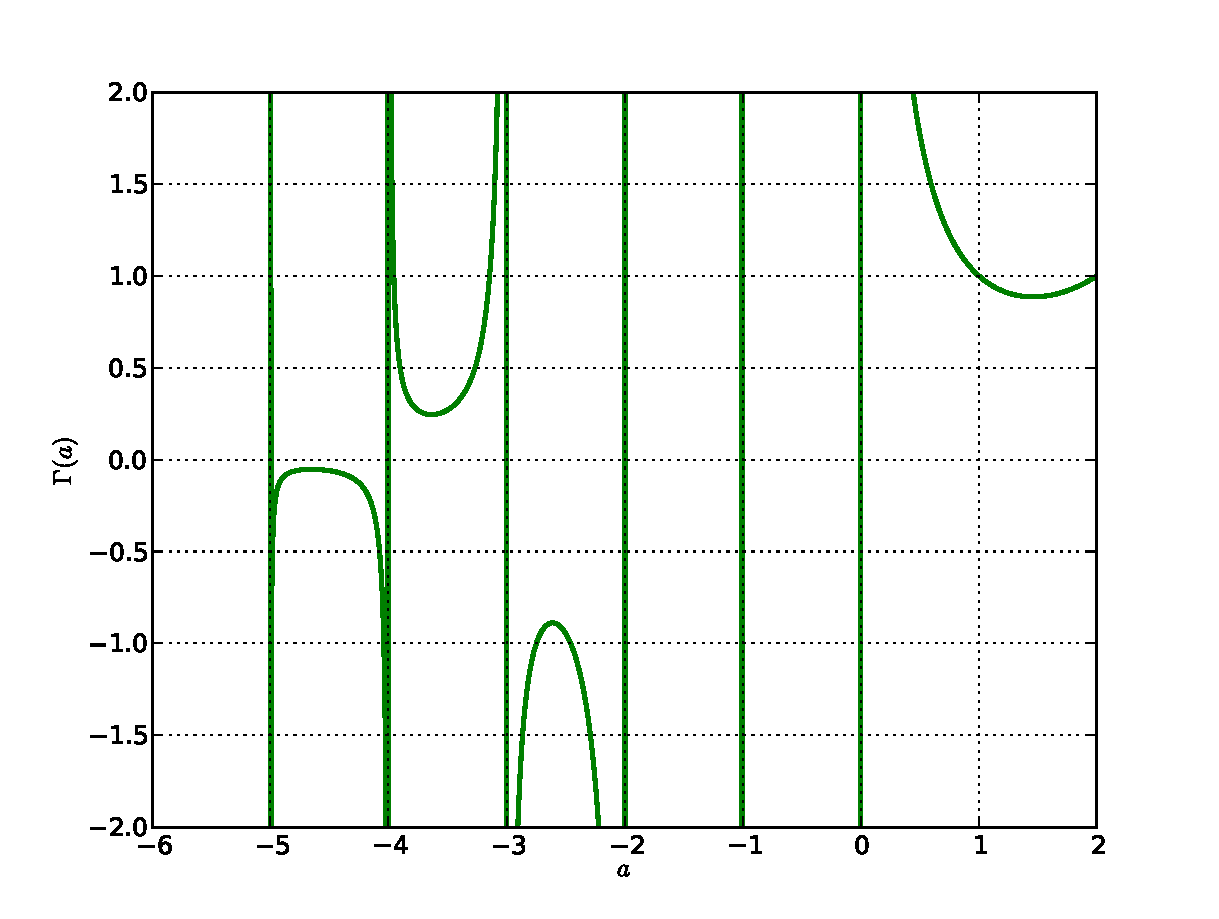
\includegraphics[width=0.5\linewidth]{gamma.pdf}
	\caption{\footnotesize{}The gamma function.}
	\label{fig:gamma}
\end{figure}
So we need an algorithm which not involves to use the gamma function for negative values. Here is described such algorithm.

\fss{Algorithm}

\fsss{Theory}

The best way to compute the incomplete gamma function for $a$ negative values is to use recurrence relations.
Let us define:
\begin{eq}
	\Gamma\pg{a+1,x}\pd=\int_x^\infty{e^{-t}{t^{a}}\dd{t}}
\end{eq}
Defining $u'=e^{-t}$ and $v=t^a$, we can use integration by parts:
\begin{eq}
	\Gamma\pg{a+1,x}\pd=\left[-e^{-t}{t^a}\right]_x^\infty + a \int_x^\infty{e^{-t}{t^{a-1}}\dd{t}}
\end{eq}
The all integrated part is always zero for all values of $a$ at infinity, and the second member of the right hand side
of the previous equation lets appear the definition of the incomplete gamma function.
So the recurrence relation for the incomplete gamma function is:
\begin{eq}
	\Gamma\pg{a+1,x}\pd=e^{-x}{x^a} + a \Gamma\pg{a,x}\pd
\end{eq}
We can see that computing the incomplete gamma function for $a<=0$ can be done with a recursive function
using the function at higher values of $a$.
\begin{eq}
	\Gamma\pg{a,x}\pd= \cfrac{ \Gamma\pg{a+1,x}\pd - e^{-x}{x^a} }{a}
\end{eq}
The previous equation shows that there is still a problem for integer values of $a$ because if $a=-2$
for example, at a moment in the recursion, we have a value of 0 for $a$ which create problems.
If we refer to \citet{abramowitz+stegun}, the definition of the elliptical integral is:
\begin{eq}
	E_n\pg{z}\pd=\int_1^\infty{e^{-zt}}{t^{-n}}\dd{t}
\end{eq}
for integer values of $n$. If we change the variable in the integral to $t'=zt$, we can rewrite the equation
to have:
\begin{eq}
	E_n\pg{z}\pd={z^{n-1}}\Gamma\pg{1-n,z}\pd
\end{eq}
so:
\begin{eq}
	\Gamma\pg{a,x}\pd={x^a}E_{1-a}\pg{x}\pd
\end{eq}
for $a\leq0$ and $a$ integer.
Now we have a good computation for the incomplete gamma function. But numerically, there is still a problem
near integer negative values of $a$. If $a$ is very close to an integer value, at a moment in the recursion,
$a$ is very small. So $1/a$ can be bigger than the overflow value for the machine. To avoid this, we add a
condition for $a$ when it is near zero.

An other definition of the incomplete gamma function is:
\begin{eq}
	\Gamma\pg{a,x}\pd=\Gamma\pg{a}\pd-\gamma\pg{a,x}\pd=\Gamma\pg{a}\pd\pg{1-P\pg{a,x}\pd}\pd
\end{eq}
with:
\begin{eq}
	\gamma\pg{a,x}\pd=\int_0^x{e^{-t}{t^{a}}\dd{t}}
\end{eq}
In \citet{NumericalRecipes} exists a precise computation of the function $P\pg{a,x}\pd$. We can remark that
this function isn't needed in the recursion if we have already access to a function which compute the
incomplete gamma function for positive values of $a$.

Following is described the algorithm for computing incomplete gamma function without loss of precision
and without numericals problems for negative values of $a$.

\fsss{Numerical}

%\begin{listing}[H]
\begin{minted}[bgcolor=griscode, linenos]{python}
def gammainc( a, x ):

	""" To compute the incomplete gamma function
	without loss of precision or without numerical
	problems. OF is the value of the overflow for
	the machine and expint( n, x ) the function
	which computes the integral function for n and x """

	import numpy as np

	if x >= 0. :

		if a <= 1. :

			if a == int( a ) or OF * abs( a ) < 1 :

				return x * int( a ) * \
					expint( 1 - int( a ), x )

			else :

				return ( gammainc( a + 1, x ) - \
					np.exp( -x ) * ( x ** a ) ) / a

		else :

			return gamma( a ) ( 1 - P( a, x ) )
			# or call the function which computes
			# the incomplete gamma function for
			# positive values of a
\end{minted}
%\end{listing}



\include{mock_ap}
\cs{Halo mass functions}

A description of how to compute halo mass functions given simple models in some articles.

\fs{Theory}

\fss{Definition}

By definition, the halo mass function by unit of comobile volume is the number of halos with mass $M$ comprise between $M$ and
$M+\dd{M}$. If $N$ is the number of halos, the halo mass function $\phi\pg{M}\pd$ can be written:
\begin{eq}
	\phi\pg{M}\pd=\cfrac{\dd{N^2}}{\dd{M}\dd{V}}=\cfrac{\dd{n}}{\dd{M}}
\end{eq}
In this case, $n$ can be the comobile density of halos, or the CDF of the density. In the latter case, we have:
\begin{eq}
	n\pg{M,z}\pd=\int_0^M{\phi\pg{M,z}\pd\dd{M}}
\end{eq}
and so:
\begin{eq}
        \frac{\dd{n}}{\dd{M}}=\frac{\dd}{\dd{M}}\int_0^M{\phi\pg{M,z}\pd}\dd{M}=\frac{\dd}{\dd{M}}\pg{\Phi\pg{M,z}\pd}-{\Phi\pg{0,z}\pd}\pd={\phi\pg{M,z}\pd}
\end{eq}
where $\Phi$ is a primitive of $\phi$.

\fss{In practice}

Cosmological simulations give results with $f\pg\sigma\pd$ a fitted function on simulations. $\sigma\pg{M}\pd$ is the variance in
mass of the smoothed density fields. We can link this function to the halo mass function by:
\begin{eq}
	\phi\pg{M,z}\pd=\frac{\dd\ln{\sigma^{-1}}}{\dd{M}}\frac{\rho_m\pg{z}\pd}{M}{f\pg\sigma\pd}=\frac{\rho_m\pg{z}\pd}{M^2}\left|{{M}\frac{\dd\ln\sigma}{\dd{M}}}\right|{f\pg\sigma\pd}
\end{eq}
where the computation of $\sigma$ involves the power spectrum $P\pg{k}\pd$ and the filter for spectrum $\tilde{W}\pg{k}\pd$:
\begin{eq}
	\sigma^2\pg{M}\pd=\cfrac{1}{2\pi^2}\int_0^\infty{P\pg{k}\pd\tilde{W}\pg{k}\pd^2{k^2}\dd{k}}
\end{eq}
This form is time consuming for the computation of the halo mass function and model dependent. In \citet{2002MNRAS.331...98V}, there
is a good approximation for this formula which is resumed to:
\begin{eq}
        \sigma(M)=\sigma_8\frac{f(u)}{f(u_8)}
\end{eq}
with the function $f$:
\begin{eq}
        f(u)=\num{64,087}{(1+\num{1,074}{u^{\num{0,3}}}-\num{1,581}{u^{\num{0,4}}}+\num{0.954}{u^{\num{0.5}}}-\num{0.185}{u^{\num{0.6}}})}^{-10}
\end{eq}
and $u$, $u_8$ which are:
\begin{eqnarray}
        u&=&\num{3.804e-4}\Gamma\left(\frac{Mh}{\Omega_{m,0}}\right)^{1/3}\nonumber\\
        u_8&=&\num{32}\Gamma\nonumber\\
        \Gamma&=&\Omega_{m,0}h\exp\left[{-\Omega_b(1+\sqrt{2h}/\Omega_{m,0})}\right]\nonumber\\
\end{eqnarray}
Now, with this approximation, we can compute easily the derivative of $\sigma$ and:
\begin{eq}
        \pg{{M}\frac{\dd\ln\sigma}{\dd{M}}}\pd^{-1}+\undemi=\frac{\left(-0.000310111 X^{1.7}+0.00225895 X^{1.6}-0.00505879 X^{1.5}-0.1 X^{1.2}\right)}{\left(-0.000328357 X^{1.8}+0.00310111 X^{1.7}-0.0090358 X^{1.6}+0.0101176 X^{1.5}\right)}
\end{eq}
with:
\comments{Check if we can used directly the power spectrum in the calculation without
too many CPU time consuming...}
\begin{eq}
        X=\left(h \Omega _{m,0} e^{-\Omega _b \left(\frac{\sqrt{2} \sqrt{h}}{\Omega _{m,0}}+1\right)} \sqrt[3]{\frac{h M}{\Omega _{m,0}}}\right)
\end{eq}

\include{form_ap}
\include{gamma_ap}

%\noindent{\rule{\linewidth}{1pt}}
%\nocite{}% permet de référencer les textes non cités
%\nocite{1999astro.ph..5116H}
%\nocite{Berstel}
\bibliographystyle{unsrtnat}
%\bibliographystyle{unsrt-fr} % permet d'avoir les textes de bibliographie en VF
%\addtocontents{toc}{\setcounter{tocdepth}{0}}
\scriptsize{\cbleu{\bibliography{/home/manuel/.texmf/tex/latex/ref.bib}}} % permet d'insérer une bibliographie
%\rule{\linewidth}{1pt}
\onecolumn
\end{sloppypar}
%\end{sloppypar}
%\clearpage
%\hypertarget{annexe}{\fs{Annexe}}
\end{document}
%###########################################################################################
% FIN DU DOCUMENT
%###########################################################################################
